% Options for packages loaded elsewhere
\PassOptionsToPackage{unicode}{hyperref}
\PassOptionsToPackage{hyphens}{url}
\documentclass[
  spanish,
]{article}
\usepackage{xcolor}
\usepackage[margin=1in]{geometry}
\usepackage{amsmath,amssymb}
\setcounter{secnumdepth}{5}
\usepackage{iftex}
\ifPDFTeX
  \usepackage[T1]{fontenc}
  \usepackage[utf8]{inputenc}
  \usepackage{textcomp} % provide euro and other symbols
\else % if luatex or xetex
  \usepackage{unicode-math} % this also loads fontspec
  \defaultfontfeatures{Scale=MatchLowercase}
  \defaultfontfeatures[\rmfamily]{Ligatures=TeX,Scale=1}
\fi
\usepackage{lmodern}
\ifPDFTeX\else
  % xetex/luatex font selection
\fi
% Use upquote if available, for straight quotes in verbatim environments
\IfFileExists{upquote.sty}{\usepackage{upquote}}{}
\IfFileExists{microtype.sty}{% use microtype if available
  \usepackage[]{microtype}
  \UseMicrotypeSet[protrusion]{basicmath} % disable protrusion for tt fonts
}{}
\makeatletter
\@ifundefined{KOMAClassName}{% if non-KOMA class
  \IfFileExists{parskip.sty}{%
    \usepackage{parskip}
  }{% else
    \setlength{\parindent}{0pt}
    \setlength{\parskip}{6pt plus 2pt minus 1pt}}
}{% if KOMA class
  \KOMAoptions{parskip=half}}
\makeatother
\usepackage{color}
\usepackage{fancyvrb}
\newcommand{\VerbBar}{|}
\newcommand{\VERB}{\Verb[commandchars=\\\{\}]}
\DefineVerbatimEnvironment{Highlighting}{Verbatim}{commandchars=\\\{\}}
% Add ',fontsize=\small' for more characters per line
\usepackage{framed}
\definecolor{shadecolor}{RGB}{248,248,248}
\newenvironment{Shaded}{\begin{snugshade}}{\end{snugshade}}
\newcommand{\AlertTok}[1]{\textcolor[rgb]{0.94,0.16,0.16}{#1}}
\newcommand{\AnnotationTok}[1]{\textcolor[rgb]{0.56,0.35,0.01}{\textbf{\textit{#1}}}}
\newcommand{\AttributeTok}[1]{\textcolor[rgb]{0.13,0.29,0.53}{#1}}
\newcommand{\BaseNTok}[1]{\textcolor[rgb]{0.00,0.00,0.81}{#1}}
\newcommand{\BuiltInTok}[1]{#1}
\newcommand{\CharTok}[1]{\textcolor[rgb]{0.31,0.60,0.02}{#1}}
\newcommand{\CommentTok}[1]{\textcolor[rgb]{0.56,0.35,0.01}{\textit{#1}}}
\newcommand{\CommentVarTok}[1]{\textcolor[rgb]{0.56,0.35,0.01}{\textbf{\textit{#1}}}}
\newcommand{\ConstantTok}[1]{\textcolor[rgb]{0.56,0.35,0.01}{#1}}
\newcommand{\ControlFlowTok}[1]{\textcolor[rgb]{0.13,0.29,0.53}{\textbf{#1}}}
\newcommand{\DataTypeTok}[1]{\textcolor[rgb]{0.13,0.29,0.53}{#1}}
\newcommand{\DecValTok}[1]{\textcolor[rgb]{0.00,0.00,0.81}{#1}}
\newcommand{\DocumentationTok}[1]{\textcolor[rgb]{0.56,0.35,0.01}{\textbf{\textit{#1}}}}
\newcommand{\ErrorTok}[1]{\textcolor[rgb]{0.64,0.00,0.00}{\textbf{#1}}}
\newcommand{\ExtensionTok}[1]{#1}
\newcommand{\FloatTok}[1]{\textcolor[rgb]{0.00,0.00,0.81}{#1}}
\newcommand{\FunctionTok}[1]{\textcolor[rgb]{0.13,0.29,0.53}{\textbf{#1}}}
\newcommand{\ImportTok}[1]{#1}
\newcommand{\InformationTok}[1]{\textcolor[rgb]{0.56,0.35,0.01}{\textbf{\textit{#1}}}}
\newcommand{\KeywordTok}[1]{\textcolor[rgb]{0.13,0.29,0.53}{\textbf{#1}}}
\newcommand{\NormalTok}[1]{#1}
\newcommand{\OperatorTok}[1]{\textcolor[rgb]{0.81,0.36,0.00}{\textbf{#1}}}
\newcommand{\OtherTok}[1]{\textcolor[rgb]{0.56,0.35,0.01}{#1}}
\newcommand{\PreprocessorTok}[1]{\textcolor[rgb]{0.56,0.35,0.01}{\textit{#1}}}
\newcommand{\RegionMarkerTok}[1]{#1}
\newcommand{\SpecialCharTok}[1]{\textcolor[rgb]{0.81,0.36,0.00}{\textbf{#1}}}
\newcommand{\SpecialStringTok}[1]{\textcolor[rgb]{0.31,0.60,0.02}{#1}}
\newcommand{\StringTok}[1]{\textcolor[rgb]{0.31,0.60,0.02}{#1}}
\newcommand{\VariableTok}[1]{\textcolor[rgb]{0.00,0.00,0.00}{#1}}
\newcommand{\VerbatimStringTok}[1]{\textcolor[rgb]{0.31,0.60,0.02}{#1}}
\newcommand{\WarningTok}[1]{\textcolor[rgb]{0.56,0.35,0.01}{\textbf{\textit{#1}}}}
\usepackage{longtable,booktabs,array}
\newcounter{none} % for unnumbered tables
\usepackage{calc} % for calculating minipage widths
% Correct order of tables after \paragraph or \subparagraph
\usepackage{etoolbox}
\makeatletter
\patchcmd\longtable{\par}{\if@noskipsec\mbox{}\fi\par}{}{}
\makeatother
% Allow footnotes in longtable head/foot
\IfFileExists{footnotehyper.sty}{\usepackage{footnotehyper}}{\usepackage{footnote}}
\makesavenoteenv{longtable}
\usepackage{graphicx}
\makeatletter
\newsavebox\pandoc@box
\newcommand*\pandocbounded[1]{% scales image to fit in text height/width
  \sbox\pandoc@box{#1}%
  \Gscale@div\@tempa{\textheight}{\dimexpr\ht\pandoc@box+\dp\pandoc@box\relax}%
  \Gscale@div\@tempb{\linewidth}{\wd\pandoc@box}%
  \ifdim\@tempb\p@<\@tempa\p@\let\@tempa\@tempb\fi% select the smaller of both
  \ifdim\@tempa\p@<\p@\scalebox{\@tempa}{\usebox\pandoc@box}%
  \else\usebox{\pandoc@box}%
  \fi%
}
% Set default figure placement to htbp
\def\fps@figure{htbp}
\makeatother
\ifLuaTeX
\usepackage[bidi=basic,shorthands=off]{babel}
\else
\usepackage[bidi=default,shorthands=off]{babel}
\fi
\ifLuaTeX
  \usepackage{selnolig} % disable illegal ligatures
\fi
\setlength{\emergencystretch}{3em} % prevent overfull lines
\providecommand{\tightlist}{%
  \setlength{\itemsep}{0pt}\setlength{\parskip}{0pt}}
\usepackage{bookmark}
\IfFileExists{xurl.sty}{\usepackage{xurl}}{} % add URL line breaks if available
\urlstyle{same}
\hypersetup{
  pdftitle={Avance del proyecto final: riesgo de pérdida en la serie GBP/USD},
  pdfauthor={{[}Nombres de los integrantes del grupo{]}},
  pdflang={es},
  hidelinks,
  pdfcreator={LaTeX via pandoc}}

\title{Avance del proyecto final: riesgo de pérdida en la serie GBP/USD}
\usepackage{etoolbox}
\makeatletter
\providecommand{\subtitle}[1]{% add subtitle to \maketitle
  \apptocmd{\@title}{\par {\large #1 \par}}{}{}
}
\makeatother
\subtitle{Computación Estadística 2026-II, Universidad Nacional de
Colombia. Grupo 2}
\author{{[}Nombres de los integrantes del grupo{]}}
\date{28 de octubre de 2026}

\begin{document}
\maketitle

\section{Introducción y datos}\label{introducciuxf3n-y-datos}

El proyecto estudia cuánto puede perderse en un día o en una semana al
mantener un activo y qué tan confiable es esa cifra. Nuestro grupo
trabaja con la serie del tipo de cambio \textbf{GBP/USD}, a partir del
archivo \texttt{retornos\_diarios\_12\_series.csv} entregado por la
docente. Según la guía, la serie cubre del 2 de enero de 1980 al 21 de
mayo de 1987 y su retorno diario es \(100\,(\ln P_t-\ln P_{t-1})\), en
porcentaje. El archivo no trae fechas, solo el número de día \(t\); el
período se toma de la guía. Se usan exclusivamente las 1866
observaciones de \texttt{GBP/USD}, que coinciden con las 1.866 que
indica la guía, con \(t\) consecutivo de 1 a 1866 y sin valores
faltantes.

Los retornos tienen media -0.0156 y desviación estándar 0.7592; su
asimetría es 0.2977 y su curtosis en exceso es 3.0563, lo que indica
colas más pesadas que las de una normal. La Figura 1 muestra que los
movimientos grandes tienden a agruparse en rachas, una señal de
volatilidad agrupada que condiciona los supuestos de independencia de
los métodos posteriores.

\textbf{Tratamiento de los ceros.} 75 retornos valen exactamente cero
(4.019 \% de la serie). Las distribuciones Weibull y lognormal solo
admiten valores estrictamente positivos, de modo que la Fase A se
construye sobre \(x_i=|r_i|\) para los \(r_i\neq 0\), que son 1791
datos. Se excluyen solo para la Fase A. En B2 se usan los retornos
originales completos, con los ceros. La consecuencia es que el modelo
ajustado nunca produce un retorno exactamente cero, mientras que en los
datos ocurre en el 4.0 \% de los días. Esto es una limitación del
modelo.

Además, el menor \(|r|\) no nulo es 0.0198, y bajo la Weibull ajustada
se esperarían unos 37 valores por debajo de ese mínimo, pero no hay
ninguno. Esto es compatible con que los precios originales estén
registrados en pasos discretos y que los movimientos muy pequeños
figuren como cero; es solo una hipótesis, que no podemos verificar con
los archivos disponibles.

\begin{figure}

{\centering 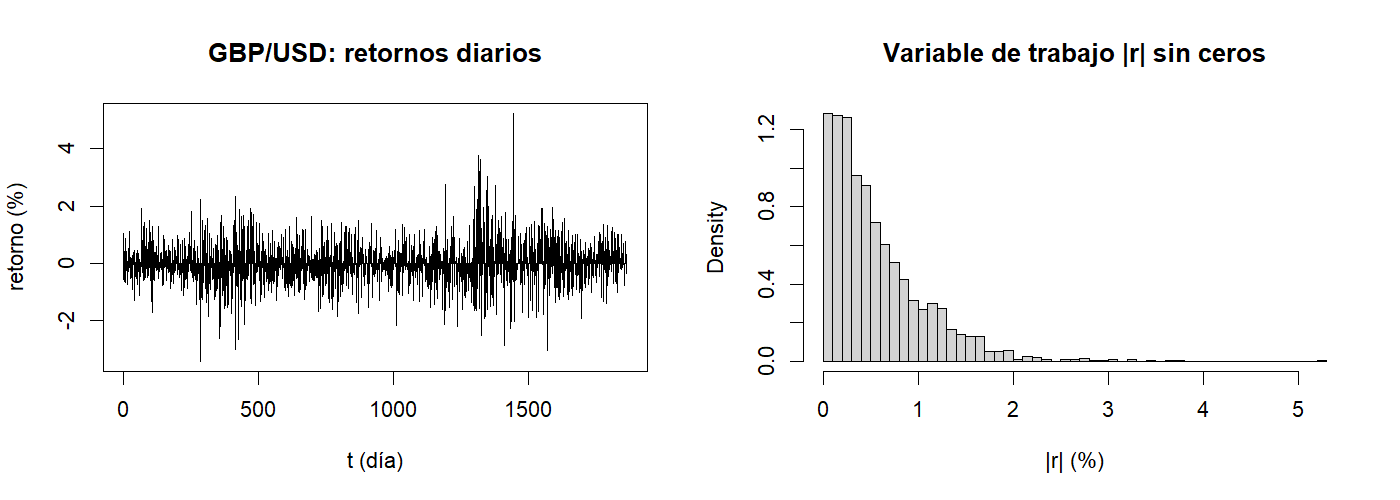
\includegraphics[width=0.92\linewidth]{figuras/01_exploracion} 

}

\caption{Retornos diarios de GBP/USD (izquierda) y variable de trabajo |r| sin ceros (derecha).}\label{fig:fig1}
\end{figure}

\section{Fase A: simulación y generación de
variables}\label{fase-a-simulaciuxf3n-y-generaciuxf3n-de-variables}

\subsection{Estimación por máxima
verosimilitud}\label{estimaciuxf3n-por-muxe1xima-verosimilitud}

Se ajustaron por máxima verosimilitud, con implementación propia, la
lognormal (solución cerrada: \(\hat\mu=\overline{\ln x}\),
\(\hat\sigma^2=\overline{(\ln x-\hat\mu)^2}\)) y la Weibull de forma
\(k\) y escala \(\lambda\). Para la Weibull,
\(\hat\lambda^k=\overline{x^k}\) y la forma \(\hat k\) es la raíz de
\[g(k)=\frac{\sum x_i^k\ln x_i}{\sum x_i^k}-\frac1k-\overline{\ln x}=0,\]
que se resolvió con el método de Newton. Como \(g'(k)>0\) para todo
\(k>0\), la raíz es única. Newton convergió en pocas iteraciones desde
varios valores iniciales. Como comprobación, \texttt{MASS::fitdistr}
(solo verificación) coincide con nuestros parámetros hasta la quinta
cifra decimal en la Weibull.

\begin{longtable}[]{@{}llrr@{}}
\caption{Parámetros estimados por máxima verosimilitud y AIC (m =
1791).}\tabularnewline
\toprule\noalign{}
Familia & Parámetros & Log-verosimilitud & AIC \\
\midrule\noalign{}
\endfirsthead
\toprule\noalign{}
Familia & Parámetros & Log-verosimilitud & AIC \\
\midrule\noalign{}
\endhead
\bottomrule\noalign{}
\endlastfoot
Lognormal & mu = -1.0035, sigma = 1.0411 & -816.10 & 1636.21 \\
Weibull & k = 1.1367, lambda = 0.5997 & -766.13 & 1536.26 \\
\end{longtable}

La Weibull tiene un AIC menor en 100.0 unidades con el mismo número de
parámetros, por lo que es la familia elegida para el resto del proyecto.
Una forma \(\hat k\approx1.14\), cercana a 1, implica una densidad que
no cae a cero en el origen, como se observa en los datos (Figura 2).

\subsection{Generación y
validación}\label{generaciuxf3n-y-validaciuxf3n}

La Weibull se simula por transformada inversa,
\(X=\lambda[-\ln U]^{1/k}\), y la lognormal con una normal estándar
generada por Box-Muller, \(X=\exp(\mu+\sigma Z)\) con
\(Z=\sqrt{-2\ln U_1}\cos(2\pi U_2)\). Solo se usa el generador uniforme
base. Se comprobó que \(F(X)\) es uniforme en la muestra Weibull y que
Box-Muller reproduce media 0 y varianza 1 con muestras grandes. Para
validar, se generó una muestra sintética 20 veces mayor que la real
(\(N=\ensuremath{3.582\times 10^{4}}\)) por familia.

\begin{figure}

{\centering 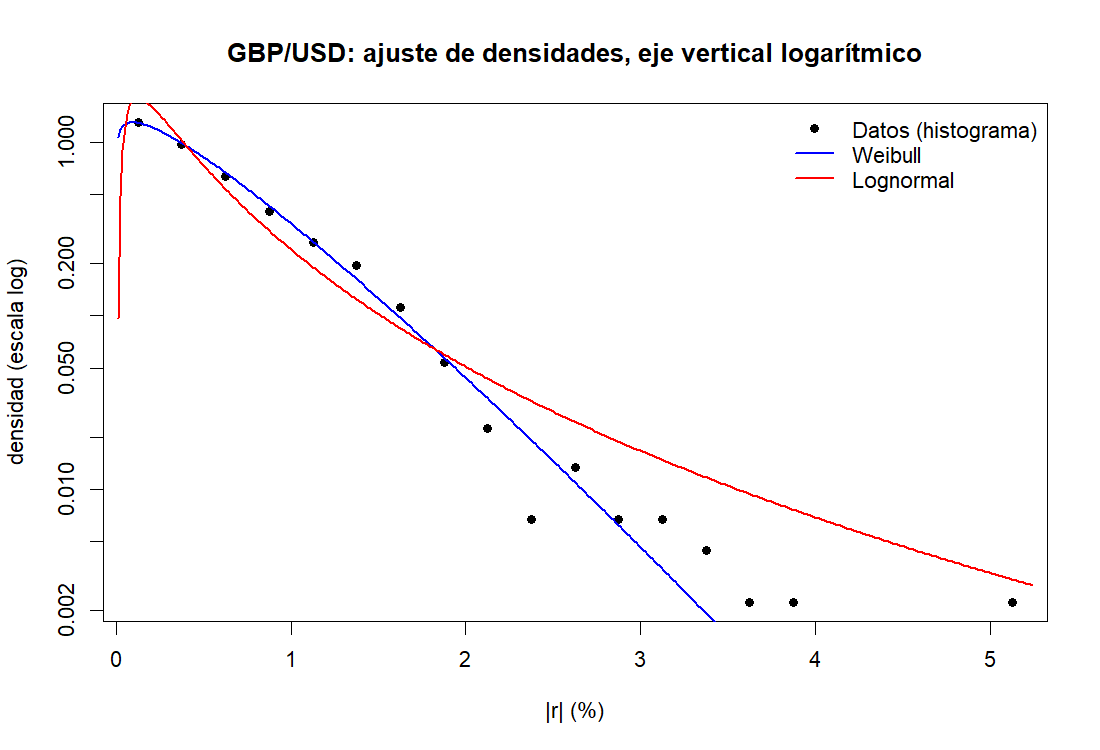
\includegraphics[width=0.92\linewidth]{figuras/02_ajuste_log} 

}

\caption{Ajuste de las densidades con eje vertical logarítmico. Cada punto aislado en la cola corresponde a muy pocas observaciones.}\label{fig:fig2}
\end{figure}

\begin{figure}

{\centering 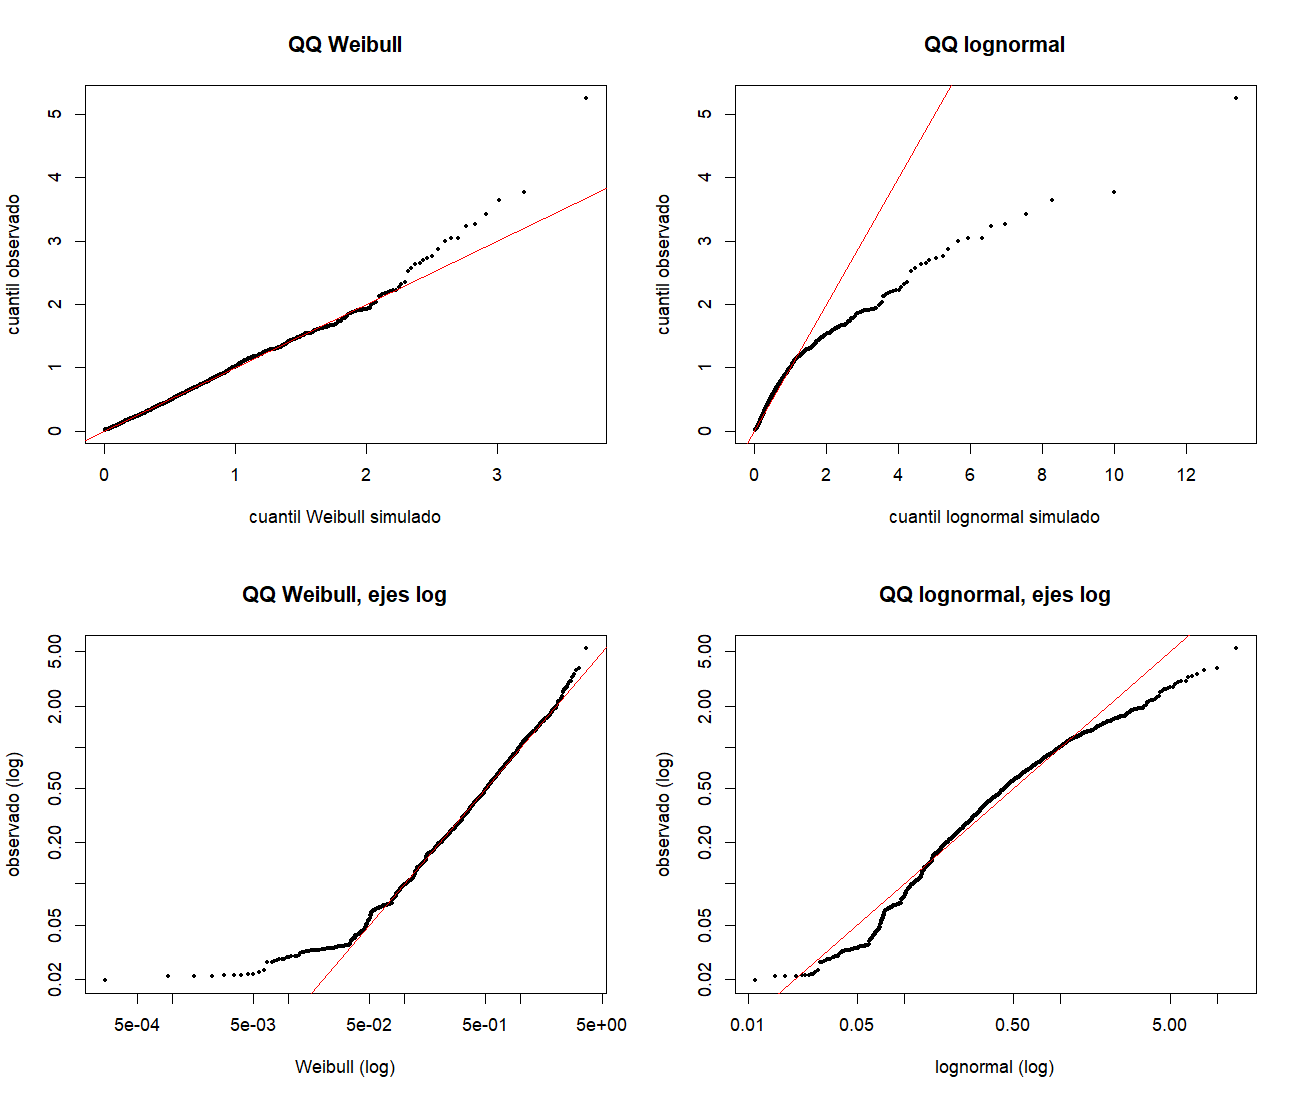
\includegraphics[width=0.92\linewidth]{figuras/03_qq} 

}

\caption{Gráficos cuantil-cuantil: cuantiles observados frente a cuantiles de las muestras sintéticas (fila inferior: ejes logarítmicos).}\label{fig:fig3}
\end{figure}

\begin{longtable}[]{@{}
  >{\raggedright\arraybackslash}p{(\linewidth - 8\tabcolsep) * \real{0.1143}}
  >{\raggedleft\arraybackslash}p{(\linewidth - 8\tabcolsep) * \real{0.1429}}
  >{\raggedleft\arraybackslash}p{(\linewidth - 8\tabcolsep) * \real{0.2429}}
  >{\raggedleft\arraybackslash}p{(\linewidth - 8\tabcolsep) * \real{0.2286}}
  >{\raggedleft\arraybackslash}p{(\linewidth - 8\tabcolsep) * \real{0.2714}}@{}}
\caption{Cuantiles 50, 90 y 99 de \textbar r\textbar.}\tabularnewline
\toprule\noalign{}
\begin{minipage}[b]{\linewidth}\raggedright
Cuantil
\end{minipage} & \begin{minipage}[b]{\linewidth}\raggedleft
Observado
\end{minipage} & \begin{minipage}[b]{\linewidth}\raggedleft
Weibull simulada
\end{minipage} & \begin{minipage}[b]{\linewidth}\raggedleft
Weibull teórica
\end{minipage} & \begin{minipage}[b]{\linewidth}\raggedleft
Lognormal simulada
\end{minipage} \\
\midrule\noalign{}
\endfirsthead
\toprule\noalign{}
\begin{minipage}[b]{\linewidth}\raggedright
Cuantil
\end{minipage} & \begin{minipage}[b]{\linewidth}\raggedleft
Observado
\end{minipage} & \begin{minipage}[b]{\linewidth}\raggedleft
Weibull simulada
\end{minipage} & \begin{minipage}[b]{\linewidth}\raggedleft
Weibull teórica
\end{minipage} & \begin{minipage}[b]{\linewidth}\raggedleft
Lognormal simulada
\end{minipage} \\
\midrule\noalign{}
\endhead
\bottomrule\noalign{}
\endlastfoot
50 \% & 0.4231 & 0.4346 & 0.4344 & 0.3681 \\
90 \% & 1.2776 & 1.2513 & 1.2490 & 1.4242 \\
99 \% & 2.3257 & 2.2870 & 2.2981 & 4.2156 \\
\end{longtable}

La distancia de Kolmogorov-Smirnov, calculada manualmente entre la
muestra observada y la sintética, es 0.0221 para la Weibull y 0.0573
para la lognormal (frente a la teórica, 0.0222 y 0.0579). Como los
parámetros se estimaron con los mismos datos, estos valores se
interpretan como medidas de distancia y no como un contraste formal.

\begin{longtable}[]{@{}
  >{\raggedright\arraybackslash}p{(\linewidth - 6\tabcolsep) * \real{0.2588}}
  >{\raggedleft\arraybackslash}p{(\linewidth - 6\tabcolsep) * \real{0.0706}}
  >{\raggedleft\arraybackslash}p{(\linewidth - 6\tabcolsep) * \real{0.2471}}
  >{\raggedleft\arraybackslash}p{(\linewidth - 6\tabcolsep) * \real{0.4235}}@{}}
\caption{Excedencias de la cola bajo el modelo Weibull.}\tabularnewline
\toprule\noalign{}
\begin{minipage}[b]{\linewidth}\raggedright
Cuantil de la Weibull
\end{minipage} & \begin{minipage}[b]{\linewidth}\raggedleft
Valor
\end{minipage} & \begin{minipage}[b]{\linewidth}\raggedleft
Datos que lo superan
\end{minipage} & \begin{minipage}[b]{\linewidth}\raggedleft
Esperados si el modelo fuera exacto
\end{minipage} \\
\midrule\noalign{}
\endfirsthead
\toprule\noalign{}
\begin{minipage}[b]{\linewidth}\raggedright
Cuantil de la Weibull
\end{minipage} & \begin{minipage}[b]{\linewidth}\raggedleft
Valor
\end{minipage} & \begin{minipage}[b]{\linewidth}\raggedleft
Datos que lo superan
\end{minipage} & \begin{minipage}[b]{\linewidth}\raggedleft
Esperados si el modelo fuera exacto
\end{minipage} \\
\midrule\noalign{}
\endhead
\bottomrule\noalign{}
\endlastfoot
99 \% & 2.298 & 19 & 17.9 \\
99.5 \% & 2.600 & 15 & 9.0 \\
99.9 \% & 3.283 & 4 & 1.8 \\
\end{longtable}

\textbf{Interpretación.} La Weibull sigue de cerca a los datos en el
centro y hasta el cuantil 99 \%, mientras que la lognormal, aunque tiene
la cola teórica más pesada, la \textbf{sobreestima} con fuerza: su
cuantil 99 \% simulado es 4.22 frente a 2.33 observado. Por otro lado,
la Weibull subestima algo el extremo de la cola: en el último 0.5 \% de
los días hay más excedencias de las esperadas (Tabla 3), y el mayor
retorno absoluto observado, 5.24, es muy poco probable bajo el modelo.
Esto es relevante para el evento raro de B1.

\textbf{Retornos con signo.} Para simular retornos con signo se asigna
\(+\) o \(-\) con probabilidad 1/2, independiente de la magnitud. Es un
supuesto del modelo (simetría y signos independientes), no una propiedad
demostrada de los datos: en la muestra hay 860 retornos positivos y 931
negativos.

\section{Fase B: integración y remuestreo
(avance)}\label{fase-b-integraciuxf3n-y-remuestreo-avance}

\subsection{B1: Monte Carlo y muestreo por
importancia}\label{b1-monte-carlo-y-muestreo-por-importancia}

Se estima \(p=P(S_5>u)\), donde \(S_5\) es la pérdida acumulada de 5
días consecutivos bajo el modelo de la Fase A (pérdidas diarias
\(s_jX_j\) independientes, con \(X_j\sim\) Weibull y signos \(\pm1\)
equiprobables). Con una simulación de referencia de \(4\times10^6\)
réplicas se eligió \(u=5.67\), el cuantil 99.9 \% de \(S_5\) redondeado,
de modo que \(p\approx0.1\) \%. Una segunda simulación independiente de
\(4\times10^6\) réplicas da \(p=0.000981\) (error estándar 0.000016).

La propuesta de muestreo por importancia genera cada \(X_j\sim\)
Weibull\((k,\,c\lambda)\) con \(c=2\) y declara un día como de pérdida
con probabilidad \(q=0.85\) en vez de 1/2. El peso es
\(W=\prod_{j=1}^5 c^{k}\exp\{-(x_j/\lambda)^k+(x_j/(c\lambda))^k\}\,(0.5/q)^{N_p}(0.5/(1-q))^{5-N_p}\),
con \(N_p\) el número de días de pérdida. El estimador es el promedio de
\(\mathbf 1\{S_5>u\}W\), insesgado porque
\(E_g[\mathbf 1\{S_5>u\}W]=p\). Los parámetros \((c,q)\) se eligieron
con un piloto sobre una rejilla de propuestas.

\begin{longtable}[]{@{}lrr@{}}
\caption{Estimación de P(pérdida a 5 días \textgreater{} 5.67) con N =
100000 simulaciones por método.}\tabularnewline
\toprule\noalign{}
Método & Estimación de p & Error estándar \\
\midrule\noalign{}
\endfirsthead
\toprule\noalign{}
Método & Estimación de p & Error estándar \\
\midrule\noalign{}
\endhead
\bottomrule\noalign{}
\endlastfoot
Monte Carlo simple & 0.000980 & 9.89e-05 \\
Muestreo por importancia & 0.000991 & 1.07e-05 \\
Referencia (4e6) & 0.000980 & 1.56e-05 \\
\end{longtable}

La reducción de varianza lograda es de 85.4 veces: el muestreo por
importancia con \(N=\ensuremath{10^{5}}\) equivale a un Monte Carlo
simple de unos 8.540.000 simulaciones. Ambas estimaciones son
compatibles con la referencia (a menos de un error estándar de
diferencia combinada).

\begin{longtable}[]{@{}rrrr@{}}
\caption{Piloto de propuestas. Un cociente menor que 1 indica que la
propuesta aumenta la varianza.}\tabularnewline
\toprule\noalign{}
c & q & Estimación & Var MC / Var IS \\
\midrule\noalign{}
\endfirsthead
\toprule\noalign{}
c & q & Estimación & Var MC / Var IS \\
\midrule\noalign{}
\endhead
\bottomrule\noalign{}
\endlastfoot
0.7 & 0.50 & 0.000822 & 0.02 \\
1.0 & 0.50 & 0.001115 & 0.88 \\
2.0 & 0.50 & 0.001001 & 14.88 \\
4.0 & 0.50 & 0.000997 & 5.22 \\
8.0 & 0.50 & 0.001116 & 0.37 \\
0.7 & 0.85 & 0.000807 & 0.11 \\
1.0 & 0.85 & 0.001040 & 3.14 \\
2.0 & 0.85 & 0.000987 & 80.97 \\
4.0 & 0.85 & 0.001011 & 29.57 \\
8.0 & 0.85 & 0.000993 & 2.42 \\
\end{longtable}

El piloto ilustra por qué la propuesta debe elegirse con cuidado: con
\(c=0.7\) la varianza es mucho mayor que la del Monte Carlo simple, y
con \(c=8\) el cociente también cae por debajo de 1 (pesos muy
dispersos). Limitación: el modelo supone días independientes, lo que
contradice la volatilidad agrupada observada, y la Weibull subestima el
extremo de la cola; la probabilidad real de una racha de pérdidas podría
ser mayor que la del modelo.

\subsection{B2: bootstrap percentil
(avance)}\label{b2-bootstrap-percentil-avance}

Sobre los retornos originales, con los 75 ceros incluidos, se estudian
la desviación estándar y el VaR al 99 \% diario (cuantil 99 \% de
\(-r\)). Se usaron \(B=5000\) réplicas con remuestreo con reemplazo
programado a mano, y el intervalo percentil del 95 \% toma los cuantiles
2.5 \% y 97.5 \% de las réplicas.

\begin{longtable}[]{@{}
  >{\raggedright\arraybackslash}p{(\linewidth - 10\tabcolsep) * \real{0.1852}}
  >{\raggedleft\arraybackslash}p{(\linewidth - 10\tabcolsep) * \real{0.1358}}
  >{\raggedleft\arraybackslash}p{(\linewidth - 10\tabcolsep) * \real{0.1975}}
  >{\raggedleft\arraybackslash}p{(\linewidth - 10\tabcolsep) * \real{0.1605}}
  >{\raggedleft\arraybackslash}p{(\linewidth - 10\tabcolsep) * \real{0.1605}}
  >{\raggedleft\arraybackslash}p{(\linewidth - 10\tabcolsep) * \real{0.1605}}@{}}
\caption{Bootstrap percentil (B = 5000) sobre los retornos
originales.}\tabularnewline
\toprule\noalign{}
\begin{minipage}[b]{\linewidth}\raggedright
Estadístico
\end{minipage} & \begin{minipage}[b]{\linewidth}\raggedleft
Estimación
\end{minipage} & \begin{minipage}[b]{\linewidth}\raggedleft
Sesgo bootstrap
\end{minipage} & \begin{minipage}[b]{\linewidth}\raggedleft
EE bootstrap
\end{minipage} & \begin{minipage}[b]{\linewidth}\raggedleft
IC 95 \% inf.
\end{minipage} & \begin{minipage}[b]{\linewidth}\raggedleft
IC 95 \% sup.
\end{minipage} \\
\midrule\noalign{}
\endfirsthead
\toprule\noalign{}
\begin{minipage}[b]{\linewidth}\raggedright
Estadístico
\end{minipage} & \begin{minipage}[b]{\linewidth}\raggedleft
Estimación
\end{minipage} & \begin{minipage}[b]{\linewidth}\raggedleft
Sesgo bootstrap
\end{minipage} & \begin{minipage}[b]{\linewidth}\raggedleft
EE bootstrap
\end{minipage} & \begin{minipage}[b]{\linewidth}\raggedleft
IC 95 \% inf.
\end{minipage} & \begin{minipage}[b]{\linewidth}\raggedleft
IC 95 \% sup.
\end{minipage} \\
\midrule\noalign{}
\endhead
\bottomrule\noalign{}
\endlastfoot
Desv. estándar & 0.7592 & -0.0002 & 0.0200 & 0.7214 & 0.7984 \\
VaR 99\% & 1.9001 & 0.0148 & 0.0973 & 1.7325 & 2.1420 \\
\end{longtable}

\begin{figure}

{\centering 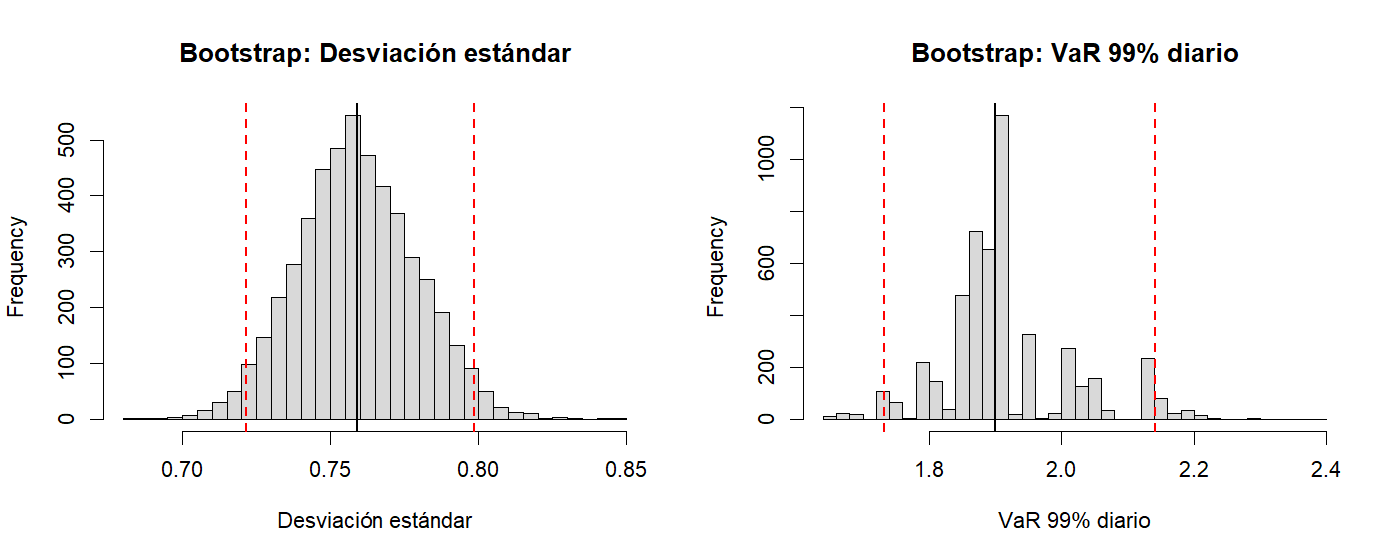
\includegraphics[width=0.92\linewidth]{figuras/04_bootstrap} 

}

\caption{Distribución bootstrap de la desviación estándar y del VaR 99 \%. La línea negra es la estimación original y las rojas, el intervalo percentil.}\label{fig:fig4}
\end{figure}

La desviación estándar es estimada con un error relativo de 2.6 \%, y su
distribución bootstrap es suave y casi simétrica. El VaR al 99 \% es
mucho menos preciso (error relativo 5.1 \%), porque depende de las pocas
pérdidas de la cola, y su distribución bootstrap es irregular: el
cuantil de una remuestra solo puede tomar valores próximos a las
pérdidas observadas más grandes, entre las que hay huecos. El sesgo
bootstrap es pequeño frente al error estándar en ambos casos. Como el
remuestreo ordinario supone observaciones independientes, estos
intervalos pueden ser demasiado optimistas si la volatilidad agrupada es
fuerte. El jackknife, el intervalo BCa y los intervalos asintóticos se
desarrollarán en la entrega final.

\section{Referencias}\label{referencias}

\begin{itemize}
\tightlist
\item
  Arel-Bundock, V. \emph{Rdatasets}.
  \url{https://github.com/vincentarelbundock/Rdatasets} (origen de los
  datos, según la guía del proyecto).
\item
  Paquete de R \texttt{Ecdat} (divisas): {[}PENDIENTE: completar autor,
  año y versión con \texttt{citation("Ecdat")}, y la referencia original
  del conjunto \texttt{Garch} que aparece en \texttt{?Garch}{]}.
\item
  Nieto Gil, Y. (2026). \emph{Guía del proyecto final, Computación
  Estadística 2026-II}. Universidad Nacional de Colombia.
\end{itemize}

\section{Nota de transparencia sobre el uso de inteligencia
artificial}\label{nota-de-transparencia-sobre-el-uso-de-inteligencia-artificial}

{[}REVISAR y ajustar por el grupo antes de entregar.{]}

\begin{itemize}
\tightlist
\item
  \textbf{Herramienta:} Claude (Anthropic), modelo Claude Sonnet 5.5,
  usado en octubre de 2026.
\item
  \textbf{Propósito:} explicar los conceptos y fórmulas de cada método,
  proponer y depurar los scripts en R, y estructurar este documento.
\item
  \textbf{Fases:} Fase A, B1 y B2 (avance).
\item
  \textbf{Verificación:} todos los scripts fueron ejecutados por el
  grupo en R; los resultados se compararon con valores de referencia
  (por ejemplo, \texttt{MASS::fitdistr} solo como verificación,
  simulación de referencia en B1) y las cifras de este documento se leen
  de los archivos generados por el código. {[}Indicar qué parte del
  código y del análisis es producto propio del grupo.{]}
\end{itemize}

\newpage

\section{Anexo: código}\label{anexo-cuxf3digo}

\subsection{funciones\_A.R}\label{funciones_a.r}

\begin{Shaded}
\begin{Highlighting}[]
\CommentTok{\# =====================================================================}
\CommentTok{\# funciones\_A.R {-} Generadores de la Fase A (SOLO definiciones, sin salida)}
\CommentTok{\# Solo se usa runif() como generador base y funciones elementales.}
\CommentTok{\# =====================================================================}

\CommentTok{\# Weibull(k forma, lam escala) por TRANSFORMADA INVERSA}
\CommentTok{\# F(x) = 1 {-} exp({-}(x/lam)\^{}k)  =\textgreater{}  F\^{}\{{-}1\}(u) = lam * ({-}log(1 {-} u))\^{}(1/k)}
\CommentTok{\# Como 1 {-} U tiene la misma distribución que U, se usa {-}log(U).}
\NormalTok{rweibull\_ti }\OtherTok{\textless{}{-}} \ControlFlowTok{function}\NormalTok{(n, k, lam) \{}
\NormalTok{  u }\OtherTok{\textless{}{-}} \FunctionTok{runif}\NormalTok{(n)}
\NormalTok{  lam }\SpecialCharTok{*}\NormalTok{ (}\SpecialCharTok{{-}}\FunctionTok{log}\NormalTok{(u))}\SpecialCharTok{\^{}}\NormalTok{(}\DecValTok{1} \SpecialCharTok{/}\NormalTok{ k)}
\NormalTok{\}}

\CommentTok{\# Normal estándar por BOX{-}MULLER (a partir de dos uniformes independientes)}
\NormalTok{rnorm\_bm }\OtherTok{\textless{}{-}} \ControlFlowTok{function}\NormalTok{(n) \{}
\NormalTok{  u1 }\OtherTok{\textless{}{-}} \FunctionTok{runif}\NormalTok{(n); u2 }\OtherTok{\textless{}{-}} \FunctionTok{runif}\NormalTok{(n)}
  \FunctionTok{sqrt}\NormalTok{(}\SpecialCharTok{{-}}\DecValTok{2} \SpecialCharTok{*} \FunctionTok{log}\NormalTok{(u1)) }\SpecialCharTok{*} \FunctionTok{cos}\NormalTok{(}\DecValTok{2} \SpecialCharTok{*}\NormalTok{ pi }\SpecialCharTok{*}\NormalTok{ u2)}
\NormalTok{\}}

\CommentTok{\# Lognormal(mu, sigma): X = exp(mu + sigma * Z), Z \textasciitilde{} N(0,1)}
\NormalTok{rlnorm\_bm }\OtherTok{\textless{}{-}} \ControlFlowTok{function}\NormalTok{(n, mu, sigma) \{}
  \FunctionTok{exp}\NormalTok{(mu }\SpecialCharTok{+}\NormalTok{ sigma }\SpecialCharTok{*} \FunctionTok{rnorm\_bm}\NormalTok{(n))}
\NormalTok{\}}

\CommentTok{\# Función de distribución acumulada de la Weibull (para verificaciones)}
\NormalTok{pweibull\_propia }\OtherTok{\textless{}{-}} \ControlFlowTok{function}\NormalTok{(x, k, lam) }\DecValTok{1} \SpecialCharTok{{-}} \FunctionTok{exp}\NormalTok{(}\SpecialCharTok{{-}}\NormalTok{(x }\SpecialCharTok{/}\NormalTok{ lam)}\SpecialCharTok{\^{}}\NormalTok{k)}

\CommentTok{\# Signos +/{-}1 con probabilidad 1/2 cada uno (supuesto del modelo, Fase A.4)}
\NormalTok{signos }\OtherTok{\textless{}{-}} \ControlFlowTok{function}\NormalTok{(n) }\FunctionTok{ifelse}\NormalTok{(}\FunctionTok{runif}\NormalTok{(n) }\SpecialCharTok{\textless{}} \FloatTok{0.5}\NormalTok{, }\DecValTok{1}\NormalTok{, }\SpecialCharTok{{-}}\DecValTok{1}\NormalTok{)}
\end{Highlighting}
\end{Shaded}

\subsection{01\_datos.R}\label{datos.r}

\begin{Shaded}
\begin{Highlighting}[]
\CommentTok{\# TAREA 1 {-} Carga de datos, ceros y variable de trabajo (GBP/USD)}
\CommentTok{\# Proyecto final {-} Computación Estadística 2026{-}II {-} GRUPO 2}
\CommentTok{\# Ejecutar desde la carpeta raíz del proyecto, con esta estructura:}
\CommentTok{\#   proyecto/}
\CommentTok{\#     data/retornos\_diarios\_12\_series.csv}
\CommentTok{\#     R/01\_datos.R}
\CommentTok{\# =====================================================================}

\FunctionTok{set.seed}\NormalTok{(}\DecValTok{2026}\NormalTok{)   }\CommentTok{\# semilla fija (aquí aún no se simula; se deja desde el inicio)}

\CommentTok{\# {-}{-}{-}{-} 1. Lectura con ruta RELATIVA {-}{-}{-}{-}{-}{-}{-}{-}{-}{-}{-}{-}{-}{-}{-}{-}{-}{-}{-}{-}{-}{-}{-}{-}{-}{-}{-}{-}{-}{-}{-}{-}{-}{-}{-}}
\NormalTok{archivo }\OtherTok{\textless{}{-}} \StringTok{"retornos\_diarios\_12\_series.csv"}
\NormalTok{candidatos }\OtherTok{\textless{}{-}} \FunctionTok{c}\NormalTok{(}\FunctionTok{file.path}\NormalTok{(}\StringTok{"data"}\NormalTok{, archivo), archivo)   }\CommentTok{\# ambas son rutas relativas}
\NormalTok{ruta }\OtherTok{\textless{}{-}}\NormalTok{ candidatos[}\FunctionTok{file.exists}\NormalTok{(candidatos)][}\DecValTok{1}\NormalTok{]}
\ControlFlowTok{if}\NormalTok{ (}\FunctionTok{is.na}\NormalTok{(ruta)) \{}
  \FunctionTok{stop}\NormalTok{(}\StringTok{"No encuentro \textquotesingle{}"}\NormalTok{, archivo, }\StringTok{"\textquotesingle{}. Carpeta de trabajo actual: "}\NormalTok{, }\FunctionTok{getwd}\NormalTok{(),}
       \StringTok{"}\SpecialCharTok{\textbackslash{}n}\StringTok{Ponga el CSV en \textquotesingle{}data/\textquotesingle{} o en esa carpeta, o cambie la carpeta de trabajo "}\NormalTok{,}
       \StringTok{"(RStudio: Session \textgreater{} Set Working Directory \textgreater{} To Source File Location)."}\NormalTok{)}
\NormalTok{\}}
\FunctionTok{cat}\NormalTok{(}\StringTok{"Leyendo:"}\NormalTok{, ruta, }\StringTok{"}\SpecialCharTok{\textbackslash{}n}\StringTok{"}\NormalTok{)}
\NormalTok{datos }\OtherTok{\textless{}{-}} \FunctionTok{read.csv}\NormalTok{(ruta, }\AttributeTok{stringsAsFactors =} \ConstantTok{FALSE}\NormalTok{, }\AttributeTok{encoding =} \StringTok{"UTF{-}8"}\NormalTok{)}

\FunctionTok{cat}\NormalTok{(}\StringTok{"Columnas:"}\NormalTok{, }\FunctionTok{names}\NormalTok{(datos), }\StringTok{"}\SpecialCharTok{\textbackslash{}n}\StringTok{"}\NormalTok{)}
\FunctionTok{cat}\NormalTok{(}\StringTok{"Series disponibles en el archivo:}\SpecialCharTok{\textbackslash{}n}\StringTok{"}\NormalTok{)}
\FunctionTok{print}\NormalTok{(}\FunctionTok{table}\NormalTok{(datos}\SpecialCharTok{$}\NormalTok{serie))}

\CommentTok{\# {-}{-}{-}{-} 2. Filtro: SOLO GBP/USD, ordenada en el tiempo {-}{-}{-}{-}{-}{-}{-}{-}{-}{-}{-}{-}{-}{-}{-}{-}{-}}
\NormalTok{gbp }\OtherTok{\textless{}{-}}\NormalTok{ datos[datos}\SpecialCharTok{$}\NormalTok{serie }\SpecialCharTok{==} \StringTok{"GBP/USD"}\NormalTok{, ]}
\NormalTok{gbp }\OtherTok{\textless{}{-}}\NormalTok{ gbp[}\FunctionTok{order}\NormalTok{(gbp}\SpecialCharTok{$}\NormalTok{t), ]}
\NormalTok{r   }\OtherTok{\textless{}{-}}\NormalTok{ gbp}\SpecialCharTok{$}\NormalTok{retorno\_pct          }\CommentTok{\# retornos originales (CON ceros): se usan en B2}

\CommentTok{\# {-}{-}{-}{-} 3. Verificaciones contra la guía {-}{-}{-}{-}{-}{-}{-}{-}{-}{-}{-}{-}{-}{-}{-}{-}{-}{-}{-}{-}{-}{-}{-}{-}{-}{-}{-}{-}{-}{-}{-}{-}}
\NormalTok{n }\OtherTok{\textless{}{-}} \FunctionTok{length}\NormalTok{(r)}
\FunctionTok{cat}\NormalTok{(}\StringTok{"}\SpecialCharTok{\textbackslash{}n}\StringTok{== Verificaciones ==}\SpecialCharTok{\textbackslash{}n}\StringTok{"}\NormalTok{)}
\FunctionTok{cat}\NormalTok{(}\StringTok{"n observaciones (guía: 1866):"}\NormalTok{, n, }\StringTok{"}\SpecialCharTok{\textbackslash{}n}\StringTok{"}\NormalTok{)}
\FunctionTok{cat}\NormalTok{(}\StringTok{"t va de"}\NormalTok{, }\FunctionTok{min}\NormalTok{(gbp}\SpecialCharTok{$}\NormalTok{t), }\StringTok{"a"}\NormalTok{, }\FunctionTok{max}\NormalTok{(gbp}\SpecialCharTok{$}\NormalTok{t), }\StringTok{"}\SpecialCharTok{\textbackslash{}n}\StringTok{"}\NormalTok{)}
\FunctionTok{cat}\NormalTok{(}\StringTok{"t consecutivo sin saltos:"}\NormalTok{, }\FunctionTok{all}\NormalTok{(}\FunctionTok{diff}\NormalTok{(gbp}\SpecialCharTok{$}\NormalTok{t) }\SpecialCharTok{==} \DecValTok{1}\NormalTok{), }\StringTok{"}\SpecialCharTok{\textbackslash{}n}\StringTok{"}\NormalTok{)}
\FunctionTok{cat}\NormalTok{(}\StringTok{"valores faltantes (NA):"}\NormalTok{, }\FunctionTok{sum}\NormalTok{(}\FunctionTok{is.na}\NormalTok{(r)), }\StringTok{"}\SpecialCharTok{\textbackslash{}n}\StringTok{"}\NormalTok{)}

\CommentTok{\# {-}{-}{-}{-} 4. Ceros exactos {-}{-}{-}{-}{-}{-}{-}{-}{-}{-}{-}{-}{-}{-}{-}{-}{-}{-}{-}{-}{-}{-}{-}{-}{-}{-}{-}{-}{-}{-}{-}{-}{-}{-}{-}{-}{-}{-}{-}{-}{-}{-}{-}{-}{-}{-}{-}{-}{-}}
\NormalTok{es\_cero  }\OtherTok{\textless{}{-}}\NormalTok{ (r }\SpecialCharTok{==} \DecValTok{0}\NormalTok{)            }\CommentTok{\# TRUE si el retorno es EXACTAMENTE 0}
\NormalTok{n\_ceros  }\OtherTok{\textless{}{-}} \FunctionTok{sum}\NormalTok{(es\_cero)}
\NormalTok{pct\_ceros }\OtherTok{\textless{}{-}} \DecValTok{100} \SpecialCharTok{*}\NormalTok{ n\_ceros }\SpecialCharTok{/}\NormalTok{ n}
\FunctionTok{cat}\NormalTok{(}\StringTok{"}\SpecialCharTok{\textbackslash{}n}\StringTok{== Ceros exactos ==}\SpecialCharTok{\textbackslash{}n}\StringTok{"}\NormalTok{)}
\FunctionTok{cat}\NormalTok{(}\StringTok{"cantidad de ceros:"}\NormalTok{, n\_ceros, }\StringTok{"}\SpecialCharTok{\textbackslash{}n}\StringTok{"}\NormalTok{)}
\FunctionTok{cat}\NormalTok{(}\FunctionTok{sprintf}\NormalTok{(}\StringTok{"porcentaje de ceros: \%.3f \%\%}\SpecialCharTok{\textbackslash{}n}\StringTok{"}\NormalTok{, pct\_ceros))}
\FunctionTok{cat}\NormalTok{(}\StringTok{"menor |r| entre los no nulos:"}\NormalTok{, }\FunctionTok{min}\NormalTok{(}\FunctionTok{abs}\NormalTok{(r[}\SpecialCharTok{!}\NormalTok{es\_cero])), }\StringTok{"}\SpecialCharTok{\textbackslash{}n}\StringTok{"}\NormalTok{)}
\FunctionTok{cat}\NormalTok{(}\StringTok{"pares de ceros en días consecutivos:"}\NormalTok{,}
    \FunctionTok{sum}\NormalTok{(es\_cero[}\SpecialCharTok{{-}}\DecValTok{1}\NormalTok{] }\SpecialCharTok{\&}\NormalTok{ es\_cero[}\SpecialCharTok{{-}}\NormalTok{n]), }\StringTok{"}\SpecialCharTok{\textbackslash{}n}\StringTok{"}\NormalTok{)}

\CommentTok{\# {-}{-}{-}{-} 5. Variable de trabajo de la Fase A: |r| sin ceros {-}{-}{-}{-}{-}{-}{-}{-}{-}{-}{-}{-}{-}}
\NormalTok{x }\OtherTok{\textless{}{-}} \FunctionTok{abs}\NormalTok{(r[}\SpecialCharTok{!}\NormalTok{es\_cero])}
\FunctionTok{cat}\NormalTok{(}\StringTok{"}\SpecialCharTok{\textbackslash{}n}\StringTok{== Variable de trabajo x = |r| (sin ceros) ==}\SpecialCharTok{\textbackslash{}n}\StringTok{"}\NormalTok{)}
\FunctionTok{cat}\NormalTok{(}\StringTok{"tamaño m:"}\NormalTok{, }\FunctionTok{length}\NormalTok{(x), }\StringTok{"}\SpecialCharTok{\textbackslash{}n}\StringTok{"}\NormalTok{)}
\FunctionTok{cat}\NormalTok{(}\StringTok{"media:"}\NormalTok{, }\FunctionTok{mean}\NormalTok{(x), }\StringTok{" desv.est.:"}\NormalTok{, }\FunctionTok{sd}\NormalTok{(x), }\StringTok{"}\SpecialCharTok{\textbackslash{}n}\StringTok{"}\NormalTok{)}
\FunctionTok{cat}\NormalTok{(}\StringTok{"mínimo:"}\NormalTok{, }\FunctionTok{min}\NormalTok{(x), }\StringTok{" máximo:"}\NormalTok{, }\FunctionTok{max}\NormalTok{(x), }\StringTok{"}\SpecialCharTok{\textbackslash{}n}\StringTok{"}\NormalTok{)}
\FunctionTok{cat}\NormalTok{(}\StringTok{"cuantiles 50, 90, 99:"}\NormalTok{, }\FunctionTok{quantile}\NormalTok{(x, }\FunctionTok{c}\NormalTok{(}\FloatTok{0.50}\NormalTok{, }\FloatTok{0.90}\NormalTok{, }\FloatTok{0.99}\NormalTok{), }\AttributeTok{type =} \DecValTok{7}\NormalTok{), }\StringTok{"}\SpecialCharTok{\textbackslash{}n}\StringTok{"}\NormalTok{)}
\FunctionTok{cat}\NormalTok{(}\StringTok{"retornos \textgreater{} 0:"}\NormalTok{, }\FunctionTok{sum}\NormalTok{(r }\SpecialCharTok{\textgreater{}} \DecValTok{0}\NormalTok{), }\StringTok{"  retornos \textless{} 0:"}\NormalTok{, }\FunctionTok{sum}\NormalTok{(r }\SpecialCharTok{\textless{}} \DecValTok{0}\NormalTok{), }\StringTok{"}\SpecialCharTok{\textbackslash{}n}\StringTok{"}\NormalTok{)}

\CommentTok{\# {-}{-}{-}{-} 6. Estadísticos descriptivos de los retornos originales {-}{-}{-}{-}{-}{-}{-}{-}}
\FunctionTok{cat}\NormalTok{(}\StringTok{"}\SpecialCharTok{\textbackslash{}n}\StringTok{== Retornos originales (con ceros) ==}\SpecialCharTok{\textbackslash{}n}\StringTok{"}\NormalTok{)}
\FunctionTok{cat}\NormalTok{(}\StringTok{"media:"}\NormalTok{, }\FunctionTok{mean}\NormalTok{(r), }\StringTok{" desv.est.:"}\NormalTok{, }\FunctionTok{sd}\NormalTok{(r), }\StringTok{"}\SpecialCharTok{\textbackslash{}n}\StringTok{"}\NormalTok{)}
\NormalTok{m2 }\OtherTok{\textless{}{-}} \FunctionTok{mean}\NormalTok{((r }\SpecialCharTok{{-}} \FunctionTok{mean}\NormalTok{(r))}\SpecialCharTok{\^{}}\DecValTok{2}\NormalTok{)}
\FunctionTok{cat}\NormalTok{(}\StringTok{"asimetría:"}\NormalTok{, }\FunctionTok{mean}\NormalTok{((r }\SpecialCharTok{{-}} \FunctionTok{mean}\NormalTok{(r))}\SpecialCharTok{\^{}}\DecValTok{3}\NormalTok{) }\SpecialCharTok{/}\NormalTok{ m2}\SpecialCharTok{\^{}}\FloatTok{1.5}\NormalTok{, }\StringTok{"}\SpecialCharTok{\textbackslash{}n}\StringTok{"}\NormalTok{)}
\FunctionTok{cat}\NormalTok{(}\StringTok{"curtosis en exceso:"}\NormalTok{, }\FunctionTok{mean}\NormalTok{((r }\SpecialCharTok{{-}} \FunctionTok{mean}\NormalTok{(r))}\SpecialCharTok{\^{}}\DecValTok{4}\NormalTok{) }\SpecialCharTok{/}\NormalTok{ m2}\SpecialCharTok{\^{}}\DecValTok{2} \SpecialCharTok{{-}} \DecValTok{3}\NormalTok{, }\StringTok{"}\SpecialCharTok{\textbackslash{}n}\StringTok{"}\NormalTok{)}

\CommentTok{\# {-}{-}{-}{-} 7. Gráfico exploratorio {-}{-}{-}{-}{-}{-}{-}{-}{-}{-}{-}{-}{-}{-}{-}{-}{-}{-}{-}{-}{-}{-}{-}{-}{-}{-}{-}{-}{-}{-}{-}{-}{-}{-}{-}{-}{-}{-}{-}{-}}
\FunctionTok{dir.create}\NormalTok{(}\StringTok{"figuras"}\NormalTok{, }\AttributeTok{showWarnings =} \ConstantTok{FALSE}\NormalTok{)}
\FunctionTok{png}\NormalTok{(}\StringTok{"figuras/01\_exploracion.png"}\NormalTok{, }\AttributeTok{width =} \DecValTok{1400}\NormalTok{, }\AttributeTok{height =} \DecValTok{500}\NormalTok{, }\AttributeTok{res =} \DecValTok{130}\NormalTok{)}
\FunctionTok{par}\NormalTok{(}\AttributeTok{mfrow =} \FunctionTok{c}\NormalTok{(}\DecValTok{1}\NormalTok{, }\DecValTok{2}\NormalTok{))}
\FunctionTok{plot}\NormalTok{(gbp}\SpecialCharTok{$}\NormalTok{t, r, }\AttributeTok{type =} \StringTok{"h"}\NormalTok{, }\AttributeTok{xlab =} \StringTok{"t (día)"}\NormalTok{, }\AttributeTok{ylab =} \StringTok{"retorno (\%)"}\NormalTok{,}
     \AttributeTok{main =} \StringTok{"GBP/USD: retornos diarios"}\NormalTok{)}
\FunctionTok{hist}\NormalTok{(x, }\AttributeTok{breaks =} \DecValTok{60}\NormalTok{, }\AttributeTok{freq =} \ConstantTok{FALSE}\NormalTok{, }\AttributeTok{xlab =} \StringTok{"|r| (\%)"}\NormalTok{,}
     \AttributeTok{main =} \StringTok{"Variable de trabajo |r| sin ceros"}\NormalTok{)}
\FunctionTok{dev.off}\NormalTok{()}
\FunctionTok{cat}\NormalTok{(}\StringTok{"}\SpecialCharTok{\textbackslash{}n}\StringTok{Figura guardada en figuras/01\_exploracion.png}\SpecialCharTok{\textbackslash{}n}\StringTok{"}\NormalTok{)}
\end{Highlighting}
\end{Shaded}

\subsection{02\_mle.R}\label{mle.r}

\begin{Shaded}
\begin{Highlighting}[]
\CommentTok{\# =====================================================================}
\CommentTok{\# TAREA 2 {-} Máxima verosimilitud: lognormal (forma cerrada) y Weibull (Newton)}
\CommentTok{\# Proyecto final {-} Computación Estadística 2026{-}II {-} GRUPO 2 {-} GBP/USD}
\CommentTok{\# Ejecutar desde la misma carpeta que 01\_datos.R (ver instrucciones previas)}
\CommentTok{\# =====================================================================}
\FunctionTok{set.seed}\NormalTok{(}\DecValTok{2026}\NormalTok{)}

\CommentTok{\# {-}{-}{-}{-} 0. Datos (mismo procedimiento de la tarea 1) {-}{-}{-}{-}{-}{-}{-}{-}{-}{-}{-}{-}{-}{-}{-}{-}{-}{-}{-}{-}}
\NormalTok{archivo }\OtherTok{\textless{}{-}} \StringTok{"retornos\_diarios\_12\_series.csv"}
\NormalTok{candidatos }\OtherTok{\textless{}{-}} \FunctionTok{c}\NormalTok{(}\FunctionTok{file.path}\NormalTok{(}\StringTok{"data"}\NormalTok{, archivo), archivo)}
\NormalTok{ruta }\OtherTok{\textless{}{-}}\NormalTok{ candidatos[}\FunctionTok{file.exists}\NormalTok{(candidatos)][}\DecValTok{1}\NormalTok{]}
\ControlFlowTok{if}\NormalTok{ (}\FunctionTok{is.na}\NormalTok{(ruta)) }\FunctionTok{stop}\NormalTok{(}\StringTok{"No encuentro el CSV. Carpeta actual: "}\NormalTok{, }\FunctionTok{getwd}\NormalTok{())}
\NormalTok{datos }\OtherTok{\textless{}{-}} \FunctionTok{read.csv}\NormalTok{(ruta, }\AttributeTok{stringsAsFactors =} \ConstantTok{FALSE}\NormalTok{, }\AttributeTok{encoding =} \StringTok{"UTF{-}8"}\NormalTok{)}
\NormalTok{gbp }\OtherTok{\textless{}{-}}\NormalTok{ datos[datos}\SpecialCharTok{$}\NormalTok{serie }\SpecialCharTok{==} \StringTok{"GBP/USD"}\NormalTok{, ]}
\NormalTok{gbp }\OtherTok{\textless{}{-}}\NormalTok{ gbp[}\FunctionTok{order}\NormalTok{(gbp}\SpecialCharTok{$}\NormalTok{t), ]}
\NormalTok{r }\OtherTok{\textless{}{-}}\NormalTok{ gbp}\SpecialCharTok{$}\NormalTok{retorno\_pct}
\NormalTok{x }\OtherTok{\textless{}{-}} \FunctionTok{abs}\NormalTok{(r[r }\SpecialCharTok{!=} \DecValTok{0}\NormalTok{])          }\CommentTok{\# variable de trabajo}
\NormalTok{m }\OtherTok{\textless{}{-}} \FunctionTok{length}\NormalTok{(x)}
\NormalTok{lx }\OtherTok{\textless{}{-}} \FunctionTok{log}\NormalTok{(x)                 }\CommentTok{\# logaritmos: se usan en ambas familias}
\FunctionTok{cat}\NormalTok{(}\StringTok{"m ="}\NormalTok{, m, }\StringTok{"}\SpecialCharTok{\textbackslash{}n}\StringTok{"}\NormalTok{)}

\CommentTok{\# {-}{-}{-}{-} 1. LOGNORMAL: solución cerrada {-}{-}{-}{-}{-}{-}{-}{-}{-}{-}{-}{-}{-}{-}{-}{-}{-}{-}{-}{-}{-}{-}{-}{-}{-}{-}{-}{-}{-}{-}{-}{-}{-}{-}}
\CommentTok{\# ln X \textasciitilde{} N(mu, sigma\^{}2)  =\textgreater{}  mu\_hat = media(ln x),  sigma2\_hat = media((ln x {-} mu\_hat)\^{}2)}
\NormalTok{mu\_ln    }\OtherTok{\textless{}{-}} \FunctionTok{mean}\NormalTok{(lx)}
\NormalTok{sigma\_ln }\OtherTok{\textless{}{-}} \FunctionTok{sqrt}\NormalTok{(}\FunctionTok{mean}\NormalTok{((lx }\SpecialCharTok{{-}}\NormalTok{ mu\_ln)}\SpecialCharTok{\^{}}\DecValTok{2}\NormalTok{))        }\CommentTok{\# divisor m (MLE), no m{-}1}

\NormalTok{loglik\_lognormal }\OtherTok{\textless{}{-}} \ControlFlowTok{function}\NormalTok{(mu, sigma, x) \{}
\NormalTok{  l }\OtherTok{\textless{}{-}} \FunctionTok{log}\NormalTok{(x)}
  \FunctionTok{sum}\NormalTok{(}\SpecialCharTok{{-}}\NormalTok{l }\SpecialCharTok{{-}} \FunctionTok{log}\NormalTok{(sigma) }\SpecialCharTok{{-}} \FloatTok{0.5} \SpecialCharTok{*} \FunctionTok{log}\NormalTok{(}\DecValTok{2} \SpecialCharTok{*}\NormalTok{ pi) }\SpecialCharTok{{-}}\NormalTok{ (l }\SpecialCharTok{{-}}\NormalTok{ mu)}\SpecialCharTok{\^{}}\DecValTok{2} \SpecialCharTok{/}\NormalTok{ (}\DecValTok{2} \SpecialCharTok{*}\NormalTok{ sigma}\SpecialCharTok{\^{}}\DecValTok{2}\NormalTok{))}
\NormalTok{\}}
\NormalTok{ll\_ln  }\OtherTok{\textless{}{-}} \FunctionTok{loglik\_lognormal}\NormalTok{(mu\_ln, sigma\_ln, x)}
\NormalTok{aic\_ln }\OtherTok{\textless{}{-}} \DecValTok{2} \SpecialCharTok{*} \DecValTok{2} \SpecialCharTok{{-}} \DecValTok{2} \SpecialCharTok{*}\NormalTok{ ll\_ln                    }\CommentTok{\# 2 parámetros}

\CommentTok{\# {-}{-}{-}{-} 2. WEIBULL: Newton para la forma k {-}{-}{-}{-}{-}{-}{-}{-}{-}{-}{-}{-}{-}{-}{-}{-}{-}{-}{-}{-}{-}{-}{-}{-}{-}{-}{-}{-}{-}{-}{-}}
\CommentTok{\# Ecuación de verosimilitud (perfil): g(k) = S1/S0 {-} 1/k {-} mean(ln x) = 0}
\CommentTok{\#   S0 = sum(x\^{}k),  S1 = sum(x\^{}k ln x),  S2 = sum(x\^{}k (ln x)\^{}2)}
\CommentTok{\# g\textquotesingle{}(k) = (S2*S0 {-} S1\^{}2)/S0\^{}2 + 1/k\^{}2}
\NormalTok{g\_weibull }\OtherTok{\textless{}{-}} \ControlFlowTok{function}\NormalTok{(k, x) \{}
\NormalTok{  l  }\OtherTok{\textless{}{-}} \FunctionTok{log}\NormalTok{(x)}
\NormalTok{  xk }\OtherTok{\textless{}{-}}\NormalTok{ x}\SpecialCharTok{\^{}}\NormalTok{k}
\NormalTok{  S0 }\OtherTok{\textless{}{-}} \FunctionTok{sum}\NormalTok{(xk); S1 }\OtherTok{\textless{}{-}} \FunctionTok{sum}\NormalTok{(xk }\SpecialCharTok{*}\NormalTok{ l); S2 }\OtherTok{\textless{}{-}} \FunctionTok{sum}\NormalTok{(xk }\SpecialCharTok{*}\NormalTok{ l}\SpecialCharTok{\^{}}\DecValTok{2}\NormalTok{)}
  \FunctionTok{c}\NormalTok{(}\AttributeTok{g  =}\NormalTok{ S1 }\SpecialCharTok{/}\NormalTok{ S0 }\SpecialCharTok{{-}} \DecValTok{1} \SpecialCharTok{/}\NormalTok{ k }\SpecialCharTok{{-}} \FunctionTok{mean}\NormalTok{(l),}
    \AttributeTok{gp =}\NormalTok{ (S2 }\SpecialCharTok{*}\NormalTok{ S0 }\SpecialCharTok{{-}}\NormalTok{ S1}\SpecialCharTok{\^{}}\DecValTok{2}\NormalTok{) }\SpecialCharTok{/}\NormalTok{ S0}\SpecialCharTok{\^{}}\DecValTok{2} \SpecialCharTok{+} \DecValTok{1} \SpecialCharTok{/}\NormalTok{ k}\SpecialCharTok{\^{}}\DecValTok{2}\NormalTok{)}
\NormalTok{\}}

\NormalTok{newton\_weibull }\OtherTok{\textless{}{-}} \ControlFlowTok{function}\NormalTok{(x, k0, }\AttributeTok{tol =} \FloatTok{1e{-}12}\NormalTok{, }\AttributeTok{max\_iter =} \DecValTok{100}\NormalTok{) \{}
\NormalTok{  k }\OtherTok{\textless{}{-}}\NormalTok{ k0}
\NormalTok{  hist }\OtherTok{\textless{}{-}} \FunctionTok{data.frame}\NormalTok{(}\AttributeTok{iter =} \DecValTok{0}\NormalTok{, }\AttributeTok{k =}\NormalTok{ k0, }\AttributeTok{g =} \FunctionTok{unname}\NormalTok{(}\FunctionTok{g\_weibull}\NormalTok{(k0, x)[}\StringTok{"g"}\NormalTok{]))}
  \ControlFlowTok{for}\NormalTok{ (it }\ControlFlowTok{in} \DecValTok{1}\SpecialCharTok{:}\NormalTok{max\_iter) \{}
\NormalTok{    v  }\OtherTok{\textless{}{-}} \FunctionTok{g\_weibull}\NormalTok{(k, x)}
\NormalTok{    kn }\OtherTok{\textless{}{-}} \FunctionTok{unname}\NormalTok{(k }\SpecialCharTok{{-}}\NormalTok{ v[}\StringTok{"g"}\NormalTok{] }\SpecialCharTok{/}\NormalTok{ v[}\StringTok{"gp"}\NormalTok{])      }\CommentTok{\# paso de Newton (unname: evita nombres heredados)}
    \ControlFlowTok{if}\NormalTok{ (}\SpecialCharTok{!}\FunctionTok{is.finite}\NormalTok{(kn) }\SpecialCharTok{||}\NormalTok{ kn }\SpecialCharTok{\textless{}=} \DecValTok{0}\NormalTok{) kn }\OtherTok{\textless{}{-}}\NormalTok{ k }\SpecialCharTok{/} \DecValTok{2}   \CommentTok{\# protección: k debe ser \textgreater{} 0}
\NormalTok{    hist }\OtherTok{\textless{}{-}} \FunctionTok{rbind}\NormalTok{(hist, }\FunctionTok{data.frame}\NormalTok{(}\AttributeTok{iter =}\NormalTok{ it, }\AttributeTok{k =} \FunctionTok{unname}\NormalTok{(kn),}
                                   \AttributeTok{g =} \FunctionTok{unname}\NormalTok{(}\FunctionTok{g\_weibull}\NormalTok{(kn, x)[}\StringTok{"g"}\NormalTok{])))}
    \ControlFlowTok{if}\NormalTok{ (}\FunctionTok{abs}\NormalTok{(kn }\SpecialCharTok{{-}}\NormalTok{ k) }\SpecialCharTok{\textless{}}\NormalTok{ tol) \{ k }\OtherTok{\textless{}{-}}\NormalTok{ kn; }\ControlFlowTok{break}\NormalTok{ \}}
\NormalTok{    k }\OtherTok{\textless{}{-}}\NormalTok{ kn}
\NormalTok{  \}}
  \FunctionTok{list}\NormalTok{(}\AttributeTok{k =} \FunctionTok{unname}\NormalTok{(k), }\AttributeTok{iter =}\NormalTok{ it, }\AttributeTok{hist =}\NormalTok{ hist)}
\NormalTok{\}}

\CommentTok{\# Valor inicial: Var(ln X) = pi\^{}2/(6 k\^{}2) para la Weibull =\textgreater{} k \textasciitilde{} 1.2 / sd(ln x)}
\CommentTok{\# (aproximación mía para arrancar; no es parte de la guía)}
\NormalTok{k0 }\OtherTok{\textless{}{-}} \FloatTok{1.2} \SpecialCharTok{/} \FunctionTok{sqrt}\NormalTok{(}\FunctionTok{mean}\NormalTok{((lx }\SpecialCharTok{{-}} \FunctionTok{mean}\NormalTok{(lx))}\SpecialCharTok{\^{}}\DecValTok{2}\NormalTok{))}
\NormalTok{nw }\OtherTok{\textless{}{-}} \FunctionTok{newton\_weibull}\NormalTok{(x, k0)}
\NormalTok{k\_w   }\OtherTok{\textless{}{-}}\NormalTok{ nw}\SpecialCharTok{$}\NormalTok{k}
\NormalTok{lam\_w }\OtherTok{\textless{}{-}}\NormalTok{ (}\FunctionTok{mean}\NormalTok{(x}\SpecialCharTok{\^{}}\NormalTok{k\_w))}\SpecialCharTok{\^{}}\NormalTok{(}\DecValTok{1} \SpecialCharTok{/}\NormalTok{ k\_w)             }\CommentTok{\# lambda\_hat\^{}k = media(x\^{}k)}

\NormalTok{loglik\_weibull }\OtherTok{\textless{}{-}} \ControlFlowTok{function}\NormalTok{(k, lam, x) \{}
\NormalTok{  m }\OtherTok{\textless{}{-}} \FunctionTok{length}\NormalTok{(x)}
\NormalTok{  m }\SpecialCharTok{*} \FunctionTok{log}\NormalTok{(k) }\SpecialCharTok{{-}}\NormalTok{ m }\SpecialCharTok{*}\NormalTok{ k }\SpecialCharTok{*} \FunctionTok{log}\NormalTok{(lam) }\SpecialCharTok{+}\NormalTok{ (k }\SpecialCharTok{{-}} \DecValTok{1}\NormalTok{) }\SpecialCharTok{*} \FunctionTok{sum}\NormalTok{(}\FunctionTok{log}\NormalTok{(x)) }\SpecialCharTok{{-}} \FunctionTok{sum}\NormalTok{((x }\SpecialCharTok{/}\NormalTok{ lam)}\SpecialCharTok{\^{}}\NormalTok{k)}
\NormalTok{\}}
\NormalTok{ll\_w  }\OtherTok{\textless{}{-}} \FunctionTok{loglik\_weibull}\NormalTok{(k\_w, lam\_w, x)}
\NormalTok{aic\_w }\OtherTok{\textless{}{-}} \DecValTok{2} \SpecialCharTok{*} \DecValTok{2} \SpecialCharTok{{-}} \DecValTok{2} \SpecialCharTok{*}\NormalTok{ ll\_w}

\FunctionTok{cat}\NormalTok{(}\StringTok{"}\SpecialCharTok{\textbackslash{}n}\StringTok{== Historial de Newton (Weibull) ==}\SpecialCharTok{\textbackslash{}n}\StringTok{"}\NormalTok{)}
\FunctionTok{print}\NormalTok{(nw}\SpecialCharTok{$}\NormalTok{hist, }\AttributeTok{row.names =} \ConstantTok{FALSE}\NormalTok{, }\AttributeTok{digits =} \DecValTok{10}\NormalTok{)}

\CommentTok{\# {-}{-}{-}{-} 3. Verificaciones propias (sin librerías) {-}{-}{-}{-}{-}{-}{-}{-}{-}{-}{-}{-}{-}{-}{-}{-}{-}{-}{-}{-}{-}{-}{-}{-}{-}}
\FunctionTok{cat}\NormalTok{(}\StringTok{"}\SpecialCharTok{\textbackslash{}n}\StringTok{== Verificaciones propias ==}\SpecialCharTok{\textbackslash{}n}\StringTok{"}\NormalTok{)}
\FunctionTok{cat}\NormalTok{(}\StringTok{"g(k\_hat) (debe ser \textasciitilde{}0):"}\NormalTok{, }\FunctionTok{g\_weibull}\NormalTok{(k\_w, x)[}\StringTok{"g"}\NormalTok{], }\StringTok{"}\SpecialCharTok{\textbackslash{}n}\StringTok{"}\NormalTok{)}
\CommentTok{\# El máximo del perfil debe estar en k\_hat: comparamos con puntos vecinos}
\NormalTok{perfil }\OtherTok{\textless{}{-}} \ControlFlowTok{function}\NormalTok{(k) \{}
\NormalTok{  lam }\OtherTok{\textless{}{-}}\NormalTok{ (}\FunctionTok{mean}\NormalTok{(x}\SpecialCharTok{\^{}}\NormalTok{k))}\SpecialCharTok{\^{}}\NormalTok{(}\DecValTok{1} \SpecialCharTok{/}\NormalTok{ k)}
  \FunctionTok{loglik\_weibull}\NormalTok{(k, lam, x)}
\NormalTok{\}}
\FunctionTok{cat}\NormalTok{(}\StringTok{"perfil en k\_hat{-}0.05, k\_hat, k\_hat+0.05:"}\NormalTok{,}
    \FunctionTok{perfil}\NormalTok{(k\_w }\SpecialCharTok{{-}} \FloatTok{0.05}\NormalTok{), }\FunctionTok{perfil}\NormalTok{(k\_w), }\FunctionTok{perfil}\NormalTok{(k\_w }\SpecialCharTok{+} \FloatTok{0.05}\NormalTok{), }\StringTok{"}\SpecialCharTok{\textbackslash{}n}\StringTok{"}\NormalTok{)}
\CommentTok{\# Robustez al valor inicial}
\ControlFlowTok{for}\NormalTok{ (k\_ini }\ControlFlowTok{in} \FunctionTok{c}\NormalTok{(}\FloatTok{0.3}\NormalTok{, }\DecValTok{1}\NormalTok{, }\DecValTok{3}\NormalTok{)) \{}
  \FunctionTok{cat}\NormalTok{(}\StringTok{"inicio"}\NormalTok{, k\_ini, }\StringTok{"{-}\textgreater{} k ="}\NormalTok{, }\FunctionTok{newton\_weibull}\NormalTok{(x, k\_ini)}\SpecialCharTok{$}\NormalTok{k, }\StringTok{"}\SpecialCharTok{\textbackslash{}n}\StringTok{"}\NormalTok{)}
\NormalTok{\}}

\CommentTok{\# {-}{-}{-}{-} 4. Tabla de resultados {-}{-}{-}{-}{-}{-}{-}{-}{-}{-}{-}{-}{-}{-}{-}{-}{-}{-}{-}{-}{-}{-}{-}{-}{-}{-}{-}{-}{-}{-}{-}{-}{-}{-}{-}{-}{-}{-}{-}{-}{-}{-}{-}{-}{-}}
\NormalTok{tabla }\OtherTok{\textless{}{-}} \FunctionTok{data.frame}\NormalTok{(}
  \AttributeTok{Familia   =} \FunctionTok{c}\NormalTok{(}\StringTok{"Lognormal"}\NormalTok{, }\StringTok{"Weibull"}\NormalTok{),}
  \AttributeTok{Parametro1 =} \FunctionTok{c}\NormalTok{(mu\_ln, k\_w),        }\CommentTok{\# lognormal: mu ; Weibull: forma k}
  \AttributeTok{Parametro2 =} \FunctionTok{c}\NormalTok{(sigma\_ln, lam\_w),   }\CommentTok{\# lognormal: sigma ; Weibull: escala lambda}
  \AttributeTok{logLik    =} \FunctionTok{c}\NormalTok{(ll\_ln, ll\_w),}
  \AttributeTok{AIC       =} \FunctionTok{c}\NormalTok{(aic\_ln, aic\_w)}
\NormalTok{)}
\FunctionTok{cat}\NormalTok{(}\StringTok{"}\SpecialCharTok{\textbackslash{}n}\StringTok{== Resultados (oficiales: implementación propia) ==}\SpecialCharTok{\textbackslash{}n}\StringTok{"}\NormalTok{)}
\FunctionTok{print}\NormalTok{(tabla, }\AttributeTok{row.names =} \ConstantTok{FALSE}\NormalTok{, }\AttributeTok{digits =} \DecValTok{8}\NormalTok{)}
\FunctionTok{cat}\NormalTok{(}\StringTok{"Lognormal: (mu, sigma) | Weibull: (k forma, lambda escala)}\SpecialCharTok{\textbackslash{}n}\StringTok{"}\NormalTok{)}
\FunctionTok{cat}\NormalTok{(}\StringTok{"Delta AIC (lognormal {-} Weibull):"}\NormalTok{, aic\_ln }\SpecialCharTok{{-}}\NormalTok{ aic\_w, }\StringTok{"}\SpecialCharTok{\textbackslash{}n}\StringTok{"}\NormalTok{)}

\CommentTok{\# {-}{-}{-}{-} 5. Comparación con librería (SOLO VERIFICACIÓN, no produce resultados) {-}{-}{-}{-}}
\FunctionTok{cat}\NormalTok{(}\StringTok{"}\SpecialCharTok{\textbackslash{}n}\StringTok{== Verificación con MASS::fitdistr (NO es el resultado oficial) ==}\SpecialCharTok{\textbackslash{}n}\StringTok{"}\NormalTok{)}
\NormalTok{res }\OtherTok{\textless{}{-}} \FunctionTok{tryCatch}\NormalTok{(\{}
\NormalTok{  f\_w  }\OtherTok{\textless{}{-}}\NormalTok{ MASS}\SpecialCharTok{::}\FunctionTok{fitdistr}\NormalTok{(x, }\StringTok{"weibull"}\NormalTok{)}
\NormalTok{  f\_ln }\OtherTok{\textless{}{-}}\NormalTok{ MASS}\SpecialCharTok{::}\FunctionTok{fitdistr}\NormalTok{(x, }\StringTok{"lognormal"}\NormalTok{)}
  \FunctionTok{print}\NormalTok{(}\FunctionTok{rbind}\NormalTok{(}
    \AttributeTok{Weibull\_propio    =} \FunctionTok{c}\NormalTok{(}\AttributeTok{forma =}\NormalTok{ k\_w, }\AttributeTok{escala =}\NormalTok{ lam\_w),}
    \AttributeTok{Weibull\_fitdistr  =} \FunctionTok{unname}\NormalTok{(f\_w}\SpecialCharTok{$}\NormalTok{estimate)}
\NormalTok{  ))}
  \FunctionTok{print}\NormalTok{(}\FunctionTok{rbind}\NormalTok{(}
    \AttributeTok{Lognormal\_propio   =} \FunctionTok{c}\NormalTok{(}\AttributeTok{meanlog =}\NormalTok{ mu\_ln, }\AttributeTok{sdlog =}\NormalTok{ sigma\_ln),}
    \AttributeTok{Lognormal\_fitdistr =} \FunctionTok{unname}\NormalTok{(f\_ln}\SpecialCharTok{$}\NormalTok{estimate)}
\NormalTok{  ))}
\NormalTok{\}, }\AttributeTok{error =} \ControlFlowTok{function}\NormalTok{(e) }\FunctionTok{cat}\NormalTok{(}\StringTok{"MASS no disponible:"}\NormalTok{, }\FunctionTok{conditionMessage}\NormalTok{(e), }\StringTok{"}\SpecialCharTok{\textbackslash{}n}\StringTok{"}\NormalTok{))}

\CommentTok{\# {-}{-}{-}{-} 6. Guardar resultados para las tareas siguientes {-}{-}{-}{-}{-}{-}{-}{-}{-}{-}{-}{-}{-}{-}{-}{-}{-}{-}{-}{-}{-}{-}}
\FunctionTok{dir.create}\NormalTok{(}\StringTok{"resultados"}\NormalTok{, }\AttributeTok{showWarnings =} \ConstantTok{FALSE}\NormalTok{)}
\FunctionTok{saveRDS}\NormalTok{(}\FunctionTok{list}\NormalTok{(}\AttributeTok{mu\_ln =}\NormalTok{ mu\_ln, }\AttributeTok{sigma\_ln =}\NormalTok{ sigma\_ln, }\AttributeTok{k\_w =}\NormalTok{ k\_w, }\AttributeTok{lam\_w =}\NormalTok{ lam\_w,}
             \AttributeTok{ll\_ln =}\NormalTok{ ll\_ln, }\AttributeTok{ll\_w =}\NormalTok{ ll\_w, }\AttributeTok{aic\_ln =}\NormalTok{ aic\_ln, }\AttributeTok{aic\_w =}\NormalTok{ aic\_w),}
        \StringTok{"resultados/params\_A.rds"}\NormalTok{)}
\FunctionTok{cat}\NormalTok{(}\StringTok{"}\SpecialCharTok{\textbackslash{}n}\StringTok{Guardado: resultados/params\_A.rds}\SpecialCharTok{\textbackslash{}n}\StringTok{"}\NormalTok{)}
\end{Highlighting}
\end{Shaded}

\subsection{03\_generadores.R}\label{generadores.r}

\begin{Shaded}
\begin{Highlighting}[]
\CommentTok{\# =====================================================================}
\CommentTok{\# TAREA 3 {-} Generadores de variables aleatorias y comprobaciones básicas}
\CommentTok{\# Proyecto final {-} Computación Estadística 2026{-}II {-} GRUPO 2 {-} GBP/USD}
\CommentTok{\# Requiere: funciones\_A.R y resultados/params\_A.rds (de 02\_mle.R)}
\CommentTok{\# =====================================================================}
\FunctionTok{set.seed}\NormalTok{(}\DecValTok{2026}\NormalTok{)}
\FunctionTok{source}\NormalTok{(}\StringTok{"funciones\_A.R"}\NormalTok{)}
\NormalTok{p }\OtherTok{\textless{}{-}} \FunctionTok{readRDS}\NormalTok{(}\StringTok{"resultados/params\_A.rds"}\NormalTok{)}
\NormalTok{k }\OtherTok{\textless{}{-}}\NormalTok{ p}\SpecialCharTok{$}\NormalTok{k\_w; lam }\OtherTok{\textless{}{-}}\NormalTok{ p}\SpecialCharTok{$}\NormalTok{lam\_w; mu }\OtherTok{\textless{}{-}}\NormalTok{ p}\SpecialCharTok{$}\NormalTok{mu\_ln; sg }\OtherTok{\textless{}{-}}\NormalTok{ p}\SpecialCharTok{$}\NormalTok{sigma\_ln}

\CommentTok{\# Tamaño de la muestra sintética: unas 20 veces el de la muestra real (m = 1791)}
\NormalTok{m  }\OtherTok{\textless{}{-}} \DecValTok{1791}
\NormalTok{N  }\OtherTok{\textless{}{-}} \DecValTok{20} \SpecialCharTok{*}\NormalTok{ m}
\FunctionTok{cat}\NormalTok{(}\StringTok{"N ="}\NormalTok{, N, }\StringTok{"}\SpecialCharTok{\textbackslash{}n}\StringTok{"}\NormalTok{)}

\CommentTok{\# {-}{-}{-}{-} 1. Normal estándar por Box{-}Muller {-}{-}{-}{-}{-}{-}{-}{-}{-}{-}{-}{-}{-}{-}{-}{-}{-}{-}{-}{-}{-}{-}{-}{-}{-}{-}{-}{-}{-}{-}{-}{-}}
\NormalTok{z }\OtherTok{\textless{}{-}} \FunctionTok{rnorm\_bm}\NormalTok{(N)}
\FunctionTok{cat}\NormalTok{(}\StringTok{"}\SpecialCharTok{\textbackslash{}n}\StringTok{== Box{-}Muller ==}\SpecialCharTok{\textbackslash{}n}\StringTok{"}\NormalTok{)}
\FunctionTok{cat}\NormalTok{(}\StringTok{"media (teórica 0):"}\NormalTok{, }\FunctionTok{mean}\NormalTok{(z), }\StringTok{"}\SpecialCharTok{\textbackslash{}n}\StringTok{"}\NormalTok{)}
\FunctionTok{cat}\NormalTok{(}\StringTok{"varianza (teórica 1):"}\NormalTok{, }\FunctionTok{mean}\NormalTok{((z }\SpecialCharTok{{-}} \FunctionTok{mean}\NormalTok{(z))}\SpecialCharTok{\^{}}\DecValTok{2}\NormalTok{), }\StringTok{"}\SpecialCharTok{\textbackslash{}n}\StringTok{"}\NormalTok{)}
\FunctionTok{cat}\NormalTok{(}\StringTok{"curtosis en exceso (teórica 0):"}\NormalTok{,}
    \FunctionTok{mean}\NormalTok{((z }\SpecialCharTok{{-}} \FunctionTok{mean}\NormalTok{(z))}\SpecialCharTok{\^{}}\DecValTok{4}\NormalTok{) }\SpecialCharTok{/} \FunctionTok{mean}\NormalTok{((z }\SpecialCharTok{{-}} \FunctionTok{mean}\NormalTok{(z))}\SpecialCharTok{\^{}}\DecValTok{2}\NormalTok{)}\SpecialCharTok{\^{}}\DecValTok{2} \SpecialCharTok{{-}} \DecValTok{3}\NormalTok{, }\StringTok{"}\SpecialCharTok{\textbackslash{}n}\StringTok{"}\NormalTok{)}

\CommentTok{\# {-}{-}{-}{-} 2. Weibull por transformada inversa {-}{-}{-}{-}{-}{-}{-}{-}{-}{-}{-}{-}{-}{-}{-}{-}{-}{-}{-}{-}{-}{-}{-}{-}{-}{-}{-}{-}{-}{-}}
\NormalTok{xw }\OtherTok{\textless{}{-}} \FunctionTok{rweibull\_ti}\NormalTok{(N, k, lam)}
\NormalTok{G  }\OtherTok{\textless{}{-}} \ControlFlowTok{function}\NormalTok{(a) }\FunctionTok{exp}\NormalTok{(}\FunctionTok{lgamma}\NormalTok{(a))                       }\CommentTok{\# Gamma(a) vía lgamma}
\NormalTok{mean\_w }\OtherTok{\textless{}{-}}\NormalTok{ lam }\SpecialCharTok{*} \FunctionTok{G}\NormalTok{(}\DecValTok{1} \SpecialCharTok{+} \DecValTok{1} \SpecialCharTok{/}\NormalTok{ k)}
\NormalTok{sd\_w   }\OtherTok{\textless{}{-}}\NormalTok{ lam }\SpecialCharTok{*} \FunctionTok{sqrt}\NormalTok{(}\FunctionTok{G}\NormalTok{(}\DecValTok{1} \SpecialCharTok{+} \DecValTok{2} \SpecialCharTok{/}\NormalTok{ k) }\SpecialCharTok{{-}} \FunctionTok{G}\NormalTok{(}\DecValTok{1} \SpecialCharTok{+} \DecValTok{1} \SpecialCharTok{/}\NormalTok{ k)}\SpecialCharTok{\^{}}\DecValTok{2}\NormalTok{)}
\NormalTok{q\_w    }\OtherTok{\textless{}{-}} \ControlFlowTok{function}\NormalTok{(pp) lam }\SpecialCharTok{*}\NormalTok{ (}\SpecialCharTok{{-}}\FunctionTok{log}\NormalTok{(}\DecValTok{1} \SpecialCharTok{{-}}\NormalTok{ pp))}\SpecialCharTok{\^{}}\NormalTok{(}\DecValTok{1} \SpecialCharTok{/}\NormalTok{ k)   }\CommentTok{\# cuantiles teóricos}
\FunctionTok{cat}\NormalTok{(}\StringTok{"}\SpecialCharTok{\textbackslash{}n}\StringTok{== Weibull (transformada inversa) ==}\SpecialCharTok{\textbackslash{}n}\StringTok{"}\NormalTok{)}
\FunctionTok{cat}\NormalTok{(}\StringTok{"media simulada / teórica:"}\NormalTok{, }\FunctionTok{mean}\NormalTok{(xw), }\StringTok{"/"}\NormalTok{, mean\_w, }\StringTok{"}\SpecialCharTok{\textbackslash{}n}\StringTok{"}\NormalTok{)}
\FunctionTok{cat}\NormalTok{(}\StringTok{"desv.est. simulada / teórica:"}\NormalTok{, }\FunctionTok{sd}\NormalTok{(xw), }\StringTok{"/"}\NormalTok{, sd\_w, }\StringTok{"}\SpecialCharTok{\textbackslash{}n}\StringTok{"}\NormalTok{)}
\FunctionTok{cat}\NormalTok{(}\StringTok{"cuantiles 50,90,99 simulados:"}\NormalTok{, }\FunctionTok{quantile}\NormalTok{(xw, }\FunctionTok{c}\NormalTok{(.}\DecValTok{5}\NormalTok{, .}\DecValTok{9}\NormalTok{, .}\DecValTok{99}\NormalTok{)), }\StringTok{"}\SpecialCharTok{\textbackslash{}n}\StringTok{"}\NormalTok{)}
\FunctionTok{cat}\NormalTok{(}\StringTok{"cuantiles 50,90,99 teóricos :"}\NormalTok{, }\FunctionTok{q\_w}\NormalTok{(}\FunctionTok{c}\NormalTok{(.}\DecValTok{5}\NormalTok{, .}\DecValTok{9}\NormalTok{, .}\DecValTok{99}\NormalTok{)), }\StringTok{"}\SpecialCharTok{\textbackslash{}n}\StringTok{"}\NormalTok{)}
\CommentTok{\# Verificación clave: F(X) debe ser Uniforme(0,1)}
\NormalTok{uu }\OtherTok{\textless{}{-}} \FunctionTok{pweibull\_propia}\NormalTok{(xw, k, lam)}
\FunctionTok{cat}\NormalTok{(}\StringTok{"F(X): media (0.5) y varianza (1/12 = 0.08333):"}\NormalTok{, }\FunctionTok{mean}\NormalTok{(uu), }\FunctionTok{mean}\NormalTok{((uu }\SpecialCharTok{{-}} \FunctionTok{mean}\NormalTok{(uu))}\SpecialCharTok{\^{}}\DecValTok{2}\NormalTok{), }\StringTok{"}\SpecialCharTok{\textbackslash{}n}\StringTok{"}\NormalTok{)}

\CommentTok{\# {-}{-}{-}{-} 3. Lognormal vía Box{-}Muller + exp(mu + sigma Z) {-}{-}{-}{-}{-}{-}{-}{-}{-}{-}{-}{-}{-}{-}{-}{-}{-}{-}{-}}
\NormalTok{xl }\OtherTok{\textless{}{-}} \FunctionTok{rlnorm\_bm}\NormalTok{(N, mu, sg)}
\FunctionTok{cat}\NormalTok{(}\StringTok{"}\SpecialCharTok{\textbackslash{}n}\StringTok{== Lognormal (Box{-}Muller) ==}\SpecialCharTok{\textbackslash{}n}\StringTok{"}\NormalTok{)}
\FunctionTok{cat}\NormalTok{(}\StringTok{"media simulada / teórica:"}\NormalTok{, }\FunctionTok{mean}\NormalTok{(xl), }\StringTok{"/"}\NormalTok{, }\FunctionTok{exp}\NormalTok{(mu }\SpecialCharTok{+}\NormalTok{ sg}\SpecialCharTok{\^{}}\DecValTok{2} \SpecialCharTok{/} \DecValTok{2}\NormalTok{), }\StringTok{"}\SpecialCharTok{\textbackslash{}n}\StringTok{"}\NormalTok{)}
\FunctionTok{cat}\NormalTok{(}\StringTok{"mediana simulada / teórica:"}\NormalTok{, }\FunctionTok{median}\NormalTok{(xl), }\StringTok{"/"}\NormalTok{, }\FunctionTok{exp}\NormalTok{(mu), }\StringTok{"}\SpecialCharTok{\textbackslash{}n}\StringTok{"}\NormalTok{)}
\FunctionTok{cat}\NormalTok{(}\StringTok{"media de ln X (mu) y desv.est. de ln X (sigma):"}\NormalTok{, }\FunctionTok{mean}\NormalTok{(}\FunctionTok{log}\NormalTok{(xl)), }\FunctionTok{sd}\NormalTok{(}\FunctionTok{log}\NormalTok{(xl)), }\StringTok{"}\SpecialCharTok{\textbackslash{}n}\StringTok{"}\NormalTok{)}

\CommentTok{\# {-}{-}{-}{-} 4. Signos {-}{-}{-}{-}{-}{-}{-}{-}{-}{-}{-}{-}{-}{-}{-}{-}{-}{-}{-}{-}{-}{-}{-}{-}{-}{-}{-}{-}{-}{-}{-}{-}{-}{-}{-}{-}{-}{-}{-}{-}{-}{-}{-}{-}{-}{-}{-}{-}{-}{-}{-}{-}{-}{-}{-}{-}{-}}
\NormalTok{s }\OtherTok{\textless{}{-}} \FunctionTok{signos}\NormalTok{(N)}
\FunctionTok{cat}\NormalTok{(}\StringTok{"}\SpecialCharTok{\textbackslash{}n}\StringTok{== Signos ==}\SpecialCharTok{\textbackslash{}n}\StringTok{"}\NormalTok{)}
\FunctionTok{cat}\NormalTok{(}\StringTok{"proporción de +1 (teórica 0.5):"}\NormalTok{, }\FunctionTok{mean}\NormalTok{(s }\SpecialCharTok{==} \DecValTok{1}\NormalTok{), }\StringTok{"}\SpecialCharTok{\textbackslash{}n}\StringTok{"}\NormalTok{)}
\FunctionTok{cat}\NormalTok{(}\StringTok{"media de los retornos simulados con signo (Weibull):"}\NormalTok{, }\FunctionTok{mean}\NormalTok{(s }\SpecialCharTok{*}\NormalTok{ xw), }\StringTok{"}\SpecialCharTok{\textbackslash{}n}\StringTok{"}\NormalTok{)}
\end{Highlighting}
\end{Shaded}

\subsection{04\_validacion.R}\label{validacion.r}

\begin{Shaded}
\begin{Highlighting}[]
\CommentTok{\# =====================================================================}
\CommentTok{\# TAREA 4 {-} Validación: gráfico de ajuste (eje log), QQ, KS a mano, cuantiles}
\CommentTok{\# Proyecto final {-} Computación Estadística 2026{-}II {-} GRUPO 2 {-} GBP/USD}
\CommentTok{\# Requiere: funciones\_A.R y resultados/params\_A.rds}
\CommentTok{\# =====================================================================}
\FunctionTok{set.seed}\NormalTok{(}\DecValTok{2026}\NormalTok{)}
\FunctionTok{source}\NormalTok{(}\StringTok{"funciones\_A.R"}\NormalTok{)}
\NormalTok{p }\OtherTok{\textless{}{-}} \FunctionTok{readRDS}\NormalTok{(}\StringTok{"resultados/params\_A.rds"}\NormalTok{)}
\NormalTok{k }\OtherTok{\textless{}{-}}\NormalTok{ p}\SpecialCharTok{$}\NormalTok{k\_w; lam }\OtherTok{\textless{}{-}}\NormalTok{ p}\SpecialCharTok{$}\NormalTok{lam\_w; mu }\OtherTok{\textless{}{-}}\NormalTok{ p}\SpecialCharTok{$}\NormalTok{mu\_ln; sg }\OtherTok{\textless{}{-}}\NormalTok{ p}\SpecialCharTok{$}\NormalTok{sigma\_ln}

\CommentTok{\# {-}{-}{-}{-} 0. Datos {-}{-}{-}{-}{-}{-}{-}{-}{-}{-}{-}{-}{-}{-}{-}{-}{-}{-}{-}{-}{-}{-}{-}{-}{-}{-}{-}{-}{-}{-}{-}{-}{-}{-}{-}{-}{-}{-}{-}{-}{-}{-}{-}{-}{-}{-}{-}{-}{-}{-}{-}{-}{-}{-}{-}{-}{-}{-}{-}{-}}
\NormalTok{archivo }\OtherTok{\textless{}{-}} \StringTok{"retornos\_diarios\_12\_series.csv"}
\NormalTok{candidatos }\OtherTok{\textless{}{-}} \FunctionTok{c}\NormalTok{(}\FunctionTok{file.path}\NormalTok{(}\StringTok{"data"}\NormalTok{, archivo), archivo)}
\NormalTok{ruta }\OtherTok{\textless{}{-}}\NormalTok{ candidatos[}\FunctionTok{file.exists}\NormalTok{(candidatos)][}\DecValTok{1}\NormalTok{]}
\ControlFlowTok{if}\NormalTok{ (}\FunctionTok{is.na}\NormalTok{(ruta)) }\FunctionTok{stop}\NormalTok{(}\StringTok{"No encuentro el CSV. Carpeta actual: "}\NormalTok{, }\FunctionTok{getwd}\NormalTok{())}
\NormalTok{datos }\OtherTok{\textless{}{-}} \FunctionTok{read.csv}\NormalTok{(ruta, }\AttributeTok{stringsAsFactors =} \ConstantTok{FALSE}\NormalTok{, }\AttributeTok{encoding =} \StringTok{"UTF{-}8"}\NormalTok{)}
\NormalTok{gbp }\OtherTok{\textless{}{-}}\NormalTok{ datos[datos}\SpecialCharTok{$}\NormalTok{serie }\SpecialCharTok{==} \StringTok{"GBP/USD"}\NormalTok{, ]; gbp }\OtherTok{\textless{}{-}}\NormalTok{ gbp[}\FunctionTok{order}\NormalTok{(gbp}\SpecialCharTok{$}\NormalTok{t), ]}
\NormalTok{r }\OtherTok{\textless{}{-}}\NormalTok{ gbp}\SpecialCharTok{$}\NormalTok{retorno\_pct}
\NormalTok{x }\OtherTok{\textless{}{-}} \FunctionTok{abs}\NormalTok{(r[r }\SpecialCharTok{!=} \DecValTok{0}\NormalTok{]); m }\OtherTok{\textless{}{-}} \FunctionTok{length}\NormalTok{(x)}
\NormalTok{xs }\OtherTok{\textless{}{-}} \FunctionTok{sort}\NormalTok{(x)                                   }\CommentTok{\# observados ordenados}

\CommentTok{\# {-}{-}{-}{-} 1. Muestras sintéticas (20 veces el tamaño de la real) {-}{-}{-}{-}{-}{-}{-}{-}{-}{-}{-}{-}{-}{-}{-}{-}}
\NormalTok{N  }\OtherTok{\textless{}{-}} \DecValTok{20} \SpecialCharTok{*}\NormalTok{ m}
\NormalTok{yw }\OtherTok{\textless{}{-}} \FunctionTok{sort}\NormalTok{(}\FunctionTok{rweibull\_ti}\NormalTok{(N, k, lam))              }\CommentTok{\# Weibull (familia elegida por AIC)}
\NormalTok{yl }\OtherTok{\textless{}{-}} \FunctionTok{sort}\NormalTok{(}\FunctionTok{rlnorm\_bm}\NormalTok{(N, mu, sg))                }\CommentTok{\# lognormal (se valida también, para comparar)}

\CommentTok{\# {-}{-}{-}{-} 2. Densidades teóricas (fórmulas propias) {-}{-}{-}{-}{-}{-}{-}{-}{-}{-}{-}{-}{-}{-}{-}{-}{-}{-}{-}{-}{-}{-}{-}{-}{-}{-}{-}{-}{-}{-}{-}{-}}
\NormalTok{dweibull\_propia }\OtherTok{\textless{}{-}} \ControlFlowTok{function}\NormalTok{(v, k, lam) (k }\SpecialCharTok{/}\NormalTok{ lam) }\SpecialCharTok{*}\NormalTok{ (v }\SpecialCharTok{/}\NormalTok{ lam)}\SpecialCharTok{\^{}}\NormalTok{(k }\SpecialCharTok{{-}} \DecValTok{1}\NormalTok{) }\SpecialCharTok{*} \FunctionTok{exp}\NormalTok{(}\SpecialCharTok{{-}}\NormalTok{(v }\SpecialCharTok{/}\NormalTok{ lam)}\SpecialCharTok{\^{}}\NormalTok{k)}
\NormalTok{dlnorm\_propia   }\OtherTok{\textless{}{-}} \ControlFlowTok{function}\NormalTok{(v, mu, s) }\FunctionTok{exp}\NormalTok{(}\SpecialCharTok{{-}}\NormalTok{(}\FunctionTok{log}\NormalTok{(v) }\SpecialCharTok{{-}}\NormalTok{ mu)}\SpecialCharTok{\^{}}\DecValTok{2} \SpecialCharTok{/}\NormalTok{ (}\DecValTok{2} \SpecialCharTok{*}\NormalTok{ s}\SpecialCharTok{\^{}}\DecValTok{2}\NormalTok{)) }\SpecialCharTok{/}\NormalTok{ (v }\SpecialCharTok{*}\NormalTok{ s }\SpecialCharTok{*} \FunctionTok{sqrt}\NormalTok{(}\DecValTok{2} \SpecialCharTok{*}\NormalTok{ pi))}

\CommentTok{\# {-}{-}{-}{-} 3. Gráfico de ajuste con eje vertical logarítmico {-}{-}{-}{-}{-}{-}{-}{-}{-}{-}{-}{-}{-}{-}{-}{-}{-}{-}{-}{-}{-}{-}{-}{-}{-}{-}{-}}
\FunctionTok{dir.create}\NormalTok{(}\StringTok{"figuras"}\NormalTok{, }\AttributeTok{showWarnings =} \ConstantTok{FALSE}\NormalTok{)}
\NormalTok{h }\OtherTok{\textless{}{-}} \FunctionTok{hist}\NormalTok{(x, }\AttributeTok{breaks =} \FunctionTok{seq}\NormalTok{(}\DecValTok{0}\NormalTok{, }\FunctionTok{ceiling}\NormalTok{(}\FunctionTok{max}\NormalTok{(x) }\SpecialCharTok{*} \DecValTok{4}\NormalTok{) }\SpecialCharTok{/} \DecValTok{4}\NormalTok{, }\AttributeTok{by =} \FloatTok{0.25}\NormalTok{), }\AttributeTok{plot =} \ConstantTok{FALSE}\NormalTok{)}
\NormalTok{ok }\OtherTok{\textless{}{-}}\NormalTok{ h}\SpecialCharTok{$}\NormalTok{density }\SpecialCharTok{\textgreater{}} \DecValTok{0}                              \CommentTok{\# el log no admite densidad 0}
\NormalTok{grid\_x }\OtherTok{\textless{}{-}} \FunctionTok{seq}\NormalTok{(}\FloatTok{0.01}\NormalTok{, }\FunctionTok{max}\NormalTok{(x), }\AttributeTok{length.out =} \DecValTok{400}\NormalTok{)}
\FunctionTok{png}\NormalTok{(}\StringTok{"figuras/02\_ajuste\_log.png"}\NormalTok{, }\AttributeTok{width =} \DecValTok{1100}\NormalTok{, }\AttributeTok{height =} \DecValTok{750}\NormalTok{, }\AttributeTok{res =} \DecValTok{130}\NormalTok{)}
\FunctionTok{plot}\NormalTok{(h}\SpecialCharTok{$}\NormalTok{mids[ok], h}\SpecialCharTok{$}\NormalTok{density[ok], }\AttributeTok{log =} \StringTok{"y"}\NormalTok{, }\AttributeTok{pch =} \DecValTok{16}\NormalTok{,}
     \AttributeTok{xlab =} \StringTok{"|r| (\%)"}\NormalTok{, }\AttributeTok{ylab =} \StringTok{"densidad (escala log)"}\NormalTok{,}
     \AttributeTok{main =} \StringTok{"GBP/USD: ajuste de densidades, eje vertical logarítmico"}\NormalTok{)}
\FunctionTok{lines}\NormalTok{(grid\_x, }\FunctionTok{dweibull\_propia}\NormalTok{(grid\_x, k, lam), }\AttributeTok{lwd =} \DecValTok{2}\NormalTok{, }\AttributeTok{col =} \StringTok{"blue"}\NormalTok{)}
\FunctionTok{lines}\NormalTok{(grid\_x, }\FunctionTok{dlnorm\_propia}\NormalTok{(grid\_x, mu, sg),  }\AttributeTok{lwd =} \DecValTok{2}\NormalTok{, }\AttributeTok{col =} \StringTok{"red"}\NormalTok{)}
\FunctionTok{legend}\NormalTok{(}\StringTok{"topright"}\NormalTok{, }\FunctionTok{c}\NormalTok{(}\StringTok{"Datos (histograma)"}\NormalTok{, }\StringTok{"Weibull"}\NormalTok{, }\StringTok{"Lognormal"}\NormalTok{),}
       \AttributeTok{pch =} \FunctionTok{c}\NormalTok{(}\DecValTok{16}\NormalTok{, }\ConstantTok{NA}\NormalTok{, }\ConstantTok{NA}\NormalTok{), }\AttributeTok{lty =} \FunctionTok{c}\NormalTok{(}\ConstantTok{NA}\NormalTok{, }\DecValTok{1}\NormalTok{, }\DecValTok{1}\NormalTok{), }\AttributeTok{lwd =} \FunctionTok{c}\NormalTok{(}\ConstantTok{NA}\NormalTok{, }\DecValTok{2}\NormalTok{, }\DecValTok{2}\NormalTok{),}
       \AttributeTok{col =} \FunctionTok{c}\NormalTok{(}\StringTok{"black"}\NormalTok{, }\StringTok{"blue"}\NormalTok{, }\StringTok{"red"}\NormalTok{), }\AttributeTok{bty =} \StringTok{"n"}\NormalTok{)}
\FunctionTok{dev.off}\NormalTok{()}

\CommentTok{\# {-}{-}{-}{-} 4. QQ{-}plot (cuantiles observados vs sintéticos) {-}{-}{-}{-}{-}{-}{-}{-}{-}{-}{-}{-}{-}{-}{-}{-}{-}{-}{-}{-}{-}{-}{-}{-}{-}{-}{-}{-}{-}{-}{-}}
\NormalTok{pi\_ }\OtherTok{\textless{}{-}}\NormalTok{ (}\DecValTok{1}\SpecialCharTok{:}\NormalTok{m }\SpecialCharTok{{-}} \FloatTok{0.5}\NormalTok{) }\SpecialCharTok{/}\NormalTok{ m                           }\CommentTok{\# probabilidades de los m observados}
\NormalTok{cuant\_sint }\OtherTok{\textless{}{-}} \ControlFlowTok{function}\NormalTok{(ysorted, pp) ysorted[}\FunctionTok{ceiling}\NormalTok{(pp }\SpecialCharTok{*} \FunctionTok{length}\NormalTok{(ysorted))]}
\NormalTok{qw }\OtherTok{\textless{}{-}} \FunctionTok{cuant\_sint}\NormalTok{(yw, pi\_)}
\NormalTok{ql }\OtherTok{\textless{}{-}} \FunctionTok{cuant\_sint}\NormalTok{(yl, pi\_)}
\FunctionTok{png}\NormalTok{(}\StringTok{"figuras/03\_qq.png"}\NormalTok{, }\AttributeTok{width =} \DecValTok{1300}\NormalTok{, }\AttributeTok{height =} \DecValTok{1100}\NormalTok{, }\AttributeTok{res =} \DecValTok{130}\NormalTok{)}
\FunctionTok{par}\NormalTok{(}\AttributeTok{mfrow =} \FunctionTok{c}\NormalTok{(}\DecValTok{2}\NormalTok{, }\DecValTok{2}\NormalTok{))}
\FunctionTok{plot}\NormalTok{(qw, xs, }\AttributeTok{pch =} \DecValTok{16}\NormalTok{, }\AttributeTok{cex =} \FloatTok{0.5}\NormalTok{, }\AttributeTok{xlab =} \StringTok{"cuantil Weibull simulado"}\NormalTok{, }\AttributeTok{ylab =} \StringTok{"cuantil observado"}\NormalTok{,}
     \AttributeTok{main =} \StringTok{"QQ Weibull"}\NormalTok{); }\FunctionTok{abline}\NormalTok{(}\DecValTok{0}\NormalTok{, }\DecValTok{1}\NormalTok{, }\AttributeTok{col =} \StringTok{"red"}\NormalTok{)}
\FunctionTok{plot}\NormalTok{(ql, xs, }\AttributeTok{pch =} \DecValTok{16}\NormalTok{, }\AttributeTok{cex =} \FloatTok{0.5}\NormalTok{, }\AttributeTok{xlab =} \StringTok{"cuantil lognormal simulado"}\NormalTok{, }\AttributeTok{ylab =} \StringTok{"cuantil observado"}\NormalTok{,}
     \AttributeTok{main =} \StringTok{"QQ lognormal"}\NormalTok{); }\FunctionTok{abline}\NormalTok{(}\DecValTok{0}\NormalTok{, }\DecValTok{1}\NormalTok{, }\AttributeTok{col =} \StringTok{"red"}\NormalTok{)}
\FunctionTok{plot}\NormalTok{(qw, xs, }\AttributeTok{pch =} \DecValTok{16}\NormalTok{, }\AttributeTok{cex =} \FloatTok{0.5}\NormalTok{, }\AttributeTok{log =} \StringTok{"xy"}\NormalTok{, }\AttributeTok{xlab =} \StringTok{"Weibull (log)"}\NormalTok{, }\AttributeTok{ylab =} \StringTok{"observado (log)"}\NormalTok{,}
     \AttributeTok{main =} \StringTok{"QQ Weibull, ejes log"}\NormalTok{); }\FunctionTok{abline}\NormalTok{(}\DecValTok{0}\NormalTok{, }\DecValTok{1}\NormalTok{, }\AttributeTok{col =} \StringTok{"red"}\NormalTok{)}
\FunctionTok{plot}\NormalTok{(ql, xs, }\AttributeTok{pch =} \DecValTok{16}\NormalTok{, }\AttributeTok{cex =} \FloatTok{0.5}\NormalTok{, }\AttributeTok{log =} \StringTok{"xy"}\NormalTok{, }\AttributeTok{xlab =} \StringTok{"lognormal (log)"}\NormalTok{, }\AttributeTok{ylab =} \StringTok{"observado (log)"}\NormalTok{,}
     \AttributeTok{main =} \StringTok{"QQ lognormal, ejes log"}\NormalTok{); }\FunctionTok{abline}\NormalTok{(}\DecValTok{0}\NormalTok{, }\DecValTok{1}\NormalTok{, }\AttributeTok{col =} \StringTok{"red"}\NormalTok{)}
\FunctionTok{dev.off}\NormalTok{()}

\CommentTok{\# {-}{-}{-}{-} 5. Distancia de Kolmogorov{-}Smirnov a mano {-}{-}{-}{-}{-}{-}{-}{-}{-}{-}{-}{-}{-}{-}{-}{-}{-}{-}{-}{-}{-}{-}{-}{-}{-}{-}{-}{-}{-}{-}{-}{-}{-}{-}{-}{-}{-}{-}{-}}
\CommentTok{\# (a) Dos muestras: D = max |F\_m(t) {-} G\_N(t)| sobre todos los puntos t de ambas muestras}
\NormalTok{ks\_dos\_muestras }\OtherTok{\textless{}{-}} \ControlFlowTok{function}\NormalTok{(a, b) \{}
\NormalTok{  a }\OtherTok{\textless{}{-}} \FunctionTok{sort}\NormalTok{(a); b }\OtherTok{\textless{}{-}} \FunctionTok{sort}\NormalTok{(b)}
\NormalTok{  t }\OtherTok{\textless{}{-}} \FunctionTok{sort}\NormalTok{(}\FunctionTok{c}\NormalTok{(a, b))}
\NormalTok{  Fa }\OtherTok{\textless{}{-}} \FunctionTok{findInterval}\NormalTok{(t, a) }\SpecialCharTok{/} \FunctionTok{length}\NormalTok{(a)           }\CommentTok{\# fracción de a \textless{}= t}
\NormalTok{  Gb }\OtherTok{\textless{}{-}} \FunctionTok{findInterval}\NormalTok{(t, b) }\SpecialCharTok{/} \FunctionTok{length}\NormalTok{(b)           }\CommentTok{\# fracción de b \textless{}= t}
  \FunctionTok{max}\NormalTok{(}\FunctionTok{abs}\NormalTok{(Fa }\SpecialCharTok{{-}}\NormalTok{ Gb))}
\NormalTok{\}}
\NormalTok{D\_w }\OtherTok{\textless{}{-}} \FunctionTok{ks\_dos\_muestras}\NormalTok{(xs, yw)}
\NormalTok{D\_l }\OtherTok{\textless{}{-}} \FunctionTok{ks\_dos\_muestras}\NormalTok{(xs, yl)}

\CommentTok{\# (b) Una muestra contra la FDA teórica (extra, determinista).}
\CommentTok{\#     La FDA normal se construye con la función de error erf (permitida), programada por serie de Taylor}
\NormalTok{erf\_propia }\OtherTok{\textless{}{-}} \ControlFlowTok{function}\NormalTok{(z) \{}
\NormalTok{  n }\OtherTok{\textless{}{-}} \DecValTok{0}\SpecialCharTok{:}\DecValTok{60}\NormalTok{; fact }\OtherTok{\textless{}{-}} \FunctionTok{c}\NormalTok{(}\DecValTok{1}\NormalTok{, }\FunctionTok{cumprod}\NormalTok{(}\DecValTok{1}\SpecialCharTok{:}\DecValTok{60}\NormalTok{))}
  \FunctionTok{sapply}\NormalTok{(z, }\ControlFlowTok{function}\NormalTok{(zz) }\DecValTok{2} \SpecialCharTok{/} \FunctionTok{sqrt}\NormalTok{(pi) }\SpecialCharTok{*} \FunctionTok{sum}\NormalTok{((}\SpecialCharTok{{-}}\DecValTok{1}\NormalTok{)}\SpecialCharTok{\^{}}\NormalTok{n }\SpecialCharTok{*}\NormalTok{ zz}\SpecialCharTok{\^{}}\NormalTok{(}\DecValTok{2} \SpecialCharTok{*}\NormalTok{ n }\SpecialCharTok{+} \DecValTok{1}\NormalTok{) }\SpecialCharTok{/}\NormalTok{ (fact }\SpecialCharTok{*}\NormalTok{ (}\DecValTok{2} \SpecialCharTok{*}\NormalTok{ n }\SpecialCharTok{+} \DecValTok{1}\NormalTok{))))}
\NormalTok{\}}
\NormalTok{pnorm\_propia  }\OtherTok{\textless{}{-}} \ControlFlowTok{function}\NormalTok{(z) }\FloatTok{0.5} \SpecialCharTok{*}\NormalTok{ (}\DecValTok{1} \SpecialCharTok{+} \FunctionTok{erf\_propia}\NormalTok{(z }\SpecialCharTok{/} \FunctionTok{sqrt}\NormalTok{(}\DecValTok{2}\NormalTok{)))}
\NormalTok{plnorm\_propia }\OtherTok{\textless{}{-}} \ControlFlowTok{function}\NormalTok{(v, mu, s) }\FunctionTok{pnorm\_propia}\NormalTok{((}\FunctionTok{log}\NormalTok{(v) }\SpecialCharTok{{-}}\NormalTok{ mu) }\SpecialCharTok{/}\NormalTok{ s)}
\NormalTok{ks\_una\_muestra }\OtherTok{\textless{}{-}} \ControlFlowTok{function}\NormalTok{(xsorted, Fteo) \{}
\NormalTok{  m }\OtherTok{\textless{}{-}} \FunctionTok{length}\NormalTok{(xsorted); i }\OtherTok{\textless{}{-}} \DecValTok{1}\SpecialCharTok{:}\NormalTok{m}
  \FunctionTok{max}\NormalTok{(}\FunctionTok{max}\NormalTok{(i }\SpecialCharTok{/}\NormalTok{ m }\SpecialCharTok{{-}}\NormalTok{ Fteo), }\FunctionTok{max}\NormalTok{(Fteo }\SpecialCharTok{{-}}\NormalTok{ (i }\SpecialCharTok{{-}} \DecValTok{1}\NormalTok{) }\SpecialCharTok{/}\NormalTok{ m))}
\NormalTok{\}}
\NormalTok{D1\_w }\OtherTok{\textless{}{-}} \FunctionTok{ks\_una\_muestra}\NormalTok{(xs, }\FunctionTok{pweibull\_propia}\NormalTok{(xs, k, lam))}
\NormalTok{D1\_l }\OtherTok{\textless{}{-}} \FunctionTok{ks\_una\_muestra}\NormalTok{(xs, }\FunctionTok{plnorm\_propia}\NormalTok{(xs, mu, sg))}
\CommentTok{\# Valor crítico asintótico aproximado al 5\% (referencia; ver advertencia en el texto)}
\NormalTok{crit }\OtherTok{\textless{}{-}} \FloatTok{1.358} \SpecialCharTok{*} \FunctionTok{sqrt}\NormalTok{((m }\SpecialCharTok{+}\NormalTok{ N) }\SpecialCharTok{/}\NormalTok{ (m }\SpecialCharTok{*}\NormalTok{ N))}
\NormalTok{crit1 }\OtherTok{\textless{}{-}} \FloatTok{1.358} \SpecialCharTok{/} \FunctionTok{sqrt}\NormalTok{(m)}

\CommentTok{\# {-}{-}{-}{-} 6. Cuantiles 50, 90 y 99 {-}{-}{-}{-}{-}{-}{-}{-}{-}{-}{-}{-}{-}{-}{-}{-}{-}{-}{-}{-}{-}{-}{-}{-}{-}{-}{-}{-}{-}{-}{-}{-}{-}{-}{-}{-}{-}{-}{-}{-}{-}{-}{-}{-}{-}{-}{-}{-}{-}{-}{-}{-}{-}{-}{-}{-}{-}{-}{-}{-}}
\NormalTok{pp }\OtherTok{\textless{}{-}} \FunctionTok{c}\NormalTok{(}\FloatTok{0.50}\NormalTok{, }\FloatTok{0.90}\NormalTok{, }\FloatTok{0.99}\NormalTok{)}
\NormalTok{tabla\_q }\OtherTok{\textless{}{-}} \FunctionTok{data.frame}\NormalTok{(}
  \AttributeTok{p =}\NormalTok{ pp,}
  \AttributeTok{observado      =} \FunctionTok{quantile}\NormalTok{(x, pp, }\AttributeTok{type =} \DecValTok{7}\NormalTok{),}
  \AttributeTok{Weibull\_sint   =} \FunctionTok{cuant\_sint}\NormalTok{(yw, pp),}
  \AttributeTok{Weibull\_teo    =}\NormalTok{ lam }\SpecialCharTok{*}\NormalTok{ (}\SpecialCharTok{{-}}\FunctionTok{log}\NormalTok{(}\DecValTok{1} \SpecialCharTok{{-}}\NormalTok{ pp))}\SpecialCharTok{\^{}}\NormalTok{(}\DecValTok{1} \SpecialCharTok{/}\NormalTok{ k),}
  \AttributeTok{lognormal\_sint =} \FunctionTok{cuant\_sint}\NormalTok{(yl, pp)}
\NormalTok{)}
\FunctionTok{rownames}\NormalTok{(tabla\_q) }\OtherTok{\textless{}{-}} \ConstantTok{NULL}

\FunctionTok{cat}\NormalTok{(}\StringTok{"}\SpecialCharTok{\textbackslash{}n}\StringTok{== Distancia KS (dos muestras: observada vs sintética de tamaño"}\NormalTok{, N, }\StringTok{") ==}\SpecialCharTok{\textbackslash{}n}\StringTok{"}\NormalTok{)}
\FunctionTok{cat}\NormalTok{(}\StringTok{"Weibull  :"}\NormalTok{, D\_w, }\StringTok{"}\SpecialCharTok{\textbackslash{}n}\StringTok{Lognormal:"}\NormalTok{, D\_l, }\StringTok{"}\SpecialCharTok{\textbackslash{}n}\StringTok{"}\NormalTok{)}
\FunctionTok{cat}\NormalTok{(}\StringTok{"Valor crítico aproximado 5\% (dos muestras):"}\NormalTok{, crit, }\StringTok{"}\SpecialCharTok{\textbackslash{}n}\StringTok{"}\NormalTok{)}
\FunctionTok{cat}\NormalTok{(}\StringTok{"}\SpecialCharTok{\textbackslash{}n}\StringTok{== Distancia KS (una muestra, contra la FDA teórica) ==}\SpecialCharTok{\textbackslash{}n}\StringTok{"}\NormalTok{)}
\FunctionTok{cat}\NormalTok{(}\StringTok{"Weibull  :"}\NormalTok{, D1\_w, }\StringTok{"}\SpecialCharTok{\textbackslash{}n}\StringTok{Lognormal:"}\NormalTok{, D1\_l, }\StringTok{"}\SpecialCharTok{\textbackslash{}n}\StringTok{"}\NormalTok{)}
\FunctionTok{cat}\NormalTok{(}\StringTok{"Valor crítico aproximado 5\% (una muestra):"}\NormalTok{, crit1, }\StringTok{"}\SpecialCharTok{\textbackslash{}n}\StringTok{"}\NormalTok{)}
\FunctionTok{cat}\NormalTok{(}\StringTok{"ADVERTENCIA: los parámetros se estimaron con los mismos datos, así que el valor crítico}\SpecialCharTok{\textbackslash{}n}\StringTok{"}\NormalTok{,}
    \StringTok{"es solo una referencia; D se interpreta como medida descriptiva de distancia.}\SpecialCharTok{\textbackslash{}n}\StringTok{"}\NormalTok{)}
\FunctionTok{cat}\NormalTok{(}\StringTok{"}\SpecialCharTok{\textbackslash{}n}\StringTok{== Cuantiles 50, 90, 99 ==}\SpecialCharTok{\textbackslash{}n}\StringTok{"}\NormalTok{)}
\FunctionTok{print}\NormalTok{(tabla\_q, }\AttributeTok{digits =} \DecValTok{5}\NormalTok{)}

\FunctionTok{saveRDS}\NormalTok{(}\FunctionTok{list}\NormalTok{(}\AttributeTok{D\_w =}\NormalTok{ D\_w, }\AttributeTok{D\_l =}\NormalTok{ D\_l, }\AttributeTok{D1\_w =}\NormalTok{ D1\_w, }\AttributeTok{D1\_l =}\NormalTok{ D1\_l, }\AttributeTok{tabla\_q =}\NormalTok{ tabla\_q),}
        \StringTok{"resultados/validacion\_A.rds"}\NormalTok{)}

\CommentTok{\# {-}{-}{-}{-} 7. Chequeo de robustez de los generadores (muestra muy grande) {-}{-}{-}{-}{-}{-}{-}{-}{-}{-}{-}{-}{-}{-}{-}{-}{-}{-}{-}{-}{-}{-}}
\NormalTok{N2 }\OtherTok{\textless{}{-}} \FloatTok{2e6}
\NormalTok{z2 }\OtherTok{\textless{}{-}} \FunctionTok{rnorm\_bm}\NormalTok{(N2)}
\FunctionTok{cat}\NormalTok{(}\StringTok{"}\SpecialCharTok{\textbackslash{}n}\StringTok{== Robustez Box{-}Muller, N ="}\NormalTok{, N2, }\StringTok{"==}\SpecialCharTok{\textbackslash{}n}\StringTok{"}\NormalTok{)}
\FunctionTok{cat}\NormalTok{(}\StringTok{"media (SE \textasciitilde{}"}\NormalTok{, }\DecValTok{1} \SpecialCharTok{/} \FunctionTok{sqrt}\NormalTok{(N2), }\StringTok{"):"}\NormalTok{, }\FunctionTok{mean}\NormalTok{(z2), }\StringTok{"}\SpecialCharTok{\textbackslash{}n}\StringTok{"}\NormalTok{)}
\FunctionTok{cat}\NormalTok{(}\StringTok{"varianza (teórica 1):"}\NormalTok{, }\FunctionTok{mean}\NormalTok{((z2 }\SpecialCharTok{{-}} \FunctionTok{mean}\NormalTok{(z2))}\SpecialCharTok{\^{}}\DecValTok{2}\NormalTok{), }\StringTok{"}\SpecialCharTok{\textbackslash{}n}\StringTok{"}\NormalTok{)}
\NormalTok{w2 }\OtherTok{\textless{}{-}} \FunctionTok{sort}\NormalTok{(}\FunctionTok{rweibull\_ti}\NormalTok{(N2, k, lam))}
\NormalTok{q99\_teo }\OtherTok{\textless{}{-}}\NormalTok{ lam }\SpecialCharTok{*}\NormalTok{ (}\SpecialCharTok{{-}}\FunctionTok{log}\NormalTok{(}\FloatTok{0.01}\NormalTok{))}\SpecialCharTok{\^{}}\NormalTok{(}\DecValTok{1} \SpecialCharTok{/}\NormalTok{ k)}
\NormalTok{se\_q99  }\OtherTok{\textless{}{-}} \FunctionTok{sqrt}\NormalTok{(}\FloatTok{0.99} \SpecialCharTok{*} \FloatTok{0.01} \SpecialCharTok{/}\NormalTok{ N2) }\SpecialCharTok{/} \FunctionTok{dweibull\_propia}\NormalTok{(q99\_teo, k, lam)}
\FunctionTok{cat}\NormalTok{(}\StringTok{"Weibull q99 simulado / teórico / SE:"}\NormalTok{, }\FunctionTok{cuant\_sint}\NormalTok{(w2, }\FloatTok{0.99}\NormalTok{), }\StringTok{"/"}\NormalTok{, q99\_teo, }\StringTok{"/"}\NormalTok{, se\_q99, }\StringTok{"}\SpecialCharTok{\textbackslash{}n}\StringTok{"}\NormalTok{)}
\end{Highlighting}
\end{Shaded}

\subsection{05\_B1.R}\label{b1.r}

\begin{Shaded}
\begin{Highlighting}[]
\CommentTok{\# =====================================================================}
\CommentTok{\# B1 {-} Monte Carlo y muestreo por importancia: P(pérdida acumulada a 5 días \textgreater{} u)}
\CommentTok{\# Proyecto final {-} Computación Estadística 2026{-}II {-} GRUPO 2 {-} GBP/USD}
\CommentTok{\# Requiere: funciones\_A.R y resultados/params\_A.rds}
\CommentTok{\# Modelo (Fase A): pérdida diaria L\_j = s\_j * X\_j, con X\_j \textasciitilde{} Weibull(k, lam) iid}
\CommentTok{\#   y s\_j = +1 (pérdida) o {-}1 (ganancia) con prob 1/2, independiente de X\_j.}
\CommentTok{\#   Evento: S5 = L\_1 + ... + L\_5 \textgreater{} u}
\CommentTok{\# =====================================================================}
\FunctionTok{set.seed}\NormalTok{(}\DecValTok{2026}\NormalTok{)}
\FunctionTok{source}\NormalTok{(}\StringTok{"funciones\_A.R"}\NormalTok{)}
\NormalTok{p }\OtherTok{\textless{}{-}} \FunctionTok{readRDS}\NormalTok{(}\StringTok{"resultados/params\_A.rds"}\NormalTok{)}
\NormalTok{k }\OtherTok{\textless{}{-}}\NormalTok{ p}\SpecialCharTok{$}\NormalTok{k\_w; lam }\OtherTok{\textless{}{-}}\NormalTok{ p}\SpecialCharTok{$}\NormalTok{lam\_w}

\CommentTok{\# {-}{-}{-}{-} 1. Simulación del modelo (MC simple) en bloques para no saturar la memoria {-}{-}{-}{-}}
\NormalTok{sim\_S5 }\OtherTok{\textless{}{-}} \ControlFlowTok{function}\NormalTok{(n) \{}
\NormalTok{  X  }\OtherTok{\textless{}{-}} \FunctionTok{matrix}\NormalTok{(}\FunctionTok{rweibull\_ti}\NormalTok{(}\DecValTok{5} \SpecialCharTok{*}\NormalTok{ n, k, lam), n, }\DecValTok{5}\NormalTok{)}
\NormalTok{  Sg }\OtherTok{\textless{}{-}} \FunctionTok{matrix}\NormalTok{(}\FunctionTok{signos}\NormalTok{(}\DecValTok{5} \SpecialCharTok{*}\NormalTok{ n), n, }\DecValTok{5}\NormalTok{)}
  \FunctionTok{rowSums}\NormalTok{(X }\SpecialCharTok{*}\NormalTok{ Sg)}
\NormalTok{\}}

\CommentTok{\# {-}{-}{-}{-} 2. Simulación de referencia y elección del umbral u {-}{-}{-}{-}{-}{-}{-}{-}{-}{-}{-}{-}{-}{-}{-}{-}{-}{-}{-}{-}{-}{-}{-}{-}{-}{-}{-}{-}}
\NormalTok{bloque }\OtherTok{\textless{}{-}} \FloatTok{2e5}
\NormalTok{Sref }\OtherTok{\textless{}{-}} \FunctionTok{unlist}\NormalTok{(}\FunctionTok{lapply}\NormalTok{(}\DecValTok{1}\SpecialCharTok{:}\DecValTok{20}\NormalTok{, }\ControlFlowTok{function}\NormalTok{(i) }\FunctionTok{sim\_S5}\NormalTok{(bloque)))     }\CommentTok{\# 4.000.000 simulaciones}
\NormalTok{u0 }\OtherTok{\textless{}{-}} \FunctionTok{quantile}\NormalTok{(Sref, }\FloatTok{0.999}\NormalTok{, }\AttributeTok{type =} \DecValTok{7}\NormalTok{, }\AttributeTok{names =} \ConstantTok{FALSE}\NormalTok{)}
\NormalTok{u  }\OtherTok{\textless{}{-}} \FunctionTok{round}\NormalTok{(u0, }\DecValTok{2}\NormalTok{)                                           }\CommentTok{\# umbral redondeado}
\FunctionTok{cat}\NormalTok{(}\StringTok{"Cuantil 99.9\% de S5 en la simulación de referencia:"}\NormalTok{, u0, }\StringTok{"}\SpecialCharTok{\textbackslash{}n}\StringTok{"}\NormalTok{)}
\FunctionTok{cat}\NormalTok{(}\StringTok{"Umbral elegido u ="}\NormalTok{, u, }\StringTok{"}\SpecialCharTok{\textbackslash{}n}\StringTok{"}\NormalTok{)}
\FunctionTok{rm}\NormalTok{(Sref)}

\CommentTok{\# Referencia independiente (otra simulación) para VALIDAR la probabilidad en u}
\NormalTok{N\_ref }\OtherTok{\textless{}{-}} \FloatTok{4e6}
\NormalTok{conteo }\OtherTok{\textless{}{-}} \DecValTok{0}
\ControlFlowTok{for}\NormalTok{ (i }\ControlFlowTok{in} \DecValTok{1}\SpecialCharTok{:}\NormalTok{(N\_ref }\SpecialCharTok{/}\NormalTok{ bloque)) conteo }\OtherTok{\textless{}{-}}\NormalTok{ conteo }\SpecialCharTok{+} \FunctionTok{sum}\NormalTok{(}\FunctionTok{sim\_S5}\NormalTok{(bloque) }\SpecialCharTok{\textgreater{}}\NormalTok{ u)}
\NormalTok{p\_ref  }\OtherTok{\textless{}{-}}\NormalTok{ conteo }\SpecialCharTok{/}\NormalTok{ N\_ref}
\NormalTok{se\_ref }\OtherTok{\textless{}{-}} \FunctionTok{sqrt}\NormalTok{(p\_ref }\SpecialCharTok{*}\NormalTok{ (}\DecValTok{1} \SpecialCharTok{{-}}\NormalTok{ p\_ref) }\SpecialCharTok{/}\NormalTok{ N\_ref)}
\FunctionTok{cat}\NormalTok{(}\FunctionTok{sprintf}\NormalTok{(}\StringTok{"Probabilidad de referencia p\_ref = \%.6f (EE = \%.6f), N\_ref = \%d}\SpecialCharTok{\textbackslash{}n}\StringTok{"}\NormalTok{,}
\NormalTok{            p\_ref, se\_ref, N\_ref))}

\CommentTok{\# {-}{-}{-}{-} 3. Muestreo por importancia {-}{-}{-}{-}{-}{-}{-}{-}{-}{-}{-}{-}{-}{-}{-}{-}{-}{-}{-}{-}{-}{-}{-}{-}{-}{-}{-}{-}{-}{-}{-}{-}{-}{-}{-}{-}{-}{-}{-}{-}{-}{-}{-}{-}{-}{-}{-}{-}{-}{-}{-}{-}{-}}
\CommentTok{\# Propuesta g: X\_j \textasciitilde{} Weibull(k, c*lam) (misma forma, escala mayor) y}
\CommentTok{\#              P(día de pérdida) = q en lugar de 1/2.}
\CommentTok{\# Peso por observación: W = prod\_j [ f(x\_j)/g(x\_j) ] * (0.5/q)\^{}\{\#pérdidas\} * (0.5/(1{-}q))\^{}\{\#ganancias\}}
\CommentTok{\# con f(x)/g(x) = c\^{}k * exp( {-}(x/lam)\^{}k + (x/(c*lam))\^{}k )  (se trabaja en logaritmos)}
\NormalTok{sim\_IS }\OtherTok{\textless{}{-}} \ControlFlowTok{function}\NormalTok{(n, c, q, u) \{}
\NormalTok{  lp }\OtherTok{\textless{}{-}}\NormalTok{ c }\SpecialCharTok{*}\NormalTok{ lam}
\NormalTok{  X    }\OtherTok{\textless{}{-}} \FunctionTok{matrix}\NormalTok{(}\FunctionTok{rweibull\_ti}\NormalTok{(}\DecValTok{5} \SpecialCharTok{*}\NormalTok{ n, k, lp), n, }\DecValTok{5}\NormalTok{)}
\NormalTok{  perd }\OtherTok{\textless{}{-}} \FunctionTok{matrix}\NormalTok{(}\FunctionTok{runif}\NormalTok{(}\DecValTok{5} \SpecialCharTok{*}\NormalTok{ n) }\SpecialCharTok{\textless{}}\NormalTok{ q, n, }\DecValTok{5}\NormalTok{)                  }\CommentTok{\# TRUE: día de pérdida}
\NormalTok{  S    }\OtherTok{\textless{}{-}} \FunctionTok{rowSums}\NormalTok{(X }\SpecialCharTok{*} \FunctionTok{ifelse}\NormalTok{(perd, }\DecValTok{1}\NormalTok{, }\SpecialCharTok{{-}}\DecValTok{1}\NormalTok{))}
\NormalTok{  logwx }\OtherTok{\textless{}{-}} \FunctionTok{rowSums}\NormalTok{(k }\SpecialCharTok{*} \FunctionTok{log}\NormalTok{(c) }\SpecialCharTok{{-}}\NormalTok{ (X }\SpecialCharTok{/}\NormalTok{ lam)}\SpecialCharTok{\^{}}\NormalTok{k }\SpecialCharTok{+}\NormalTok{ (X }\SpecialCharTok{/}\NormalTok{ lp)}\SpecialCharTok{\^{}}\NormalTok{k)}
\NormalTok{  nl    }\OtherTok{\textless{}{-}} \FunctionTok{rowSums}\NormalTok{(perd)}
\NormalTok{  logws }\OtherTok{\textless{}{-}}\NormalTok{ nl }\SpecialCharTok{*} \FunctionTok{log}\NormalTok{(}\FloatTok{0.5} \SpecialCharTok{/}\NormalTok{ q) }\SpecialCharTok{+}\NormalTok{ (}\DecValTok{5} \SpecialCharTok{{-}}\NormalTok{ nl) }\SpecialCharTok{*} \FunctionTok{log}\NormalTok{(}\FloatTok{0.5} \SpecialCharTok{/}\NormalTok{ (}\DecValTok{1} \SpecialCharTok{{-}}\NormalTok{ q))}
\NormalTok{  logw  }\OtherTok{\textless{}{-}}\NormalTok{ logwx }\SpecialCharTok{+}\NormalTok{ logws}
\NormalTok{  y }\OtherTok{\textless{}{-}} \FunctionTok{numeric}\NormalTok{(n)}
\NormalTok{  idx }\OtherTok{\textless{}{-}} \FunctionTok{which}\NormalTok{(S }\SpecialCharTok{\textgreater{}}\NormalTok{ u)}
\NormalTok{  y[idx] }\OtherTok{\textless{}{-}} \FunctionTok{exp}\NormalTok{(logw[idx])                                }\CommentTok{\# indicador * peso}
  \FunctionTok{list}\NormalTok{(}\AttributeTok{y =}\NormalTok{ y, }\AttributeTok{logw =}\NormalTok{ logw)}
\NormalTok{\}}

\CommentTok{\# {-}{-}{-}{-} 4. Estudio piloto: cómo elegir la propuesta (y qué pasa si se elige mal) {-}{-}{-}{-}{-}{-}{-}{-}{-}{-}}
\FunctionTok{cat}\NormalTok{(}\StringTok{"}\SpecialCharTok{\textbackslash{}n}\StringTok{== Piloto (n = 2e5 por combinación) ==}\SpecialCharTok{\textbackslash{}n}\StringTok{"}\NormalTok{)}
\NormalTok{cs }\OtherTok{\textless{}{-}} \FunctionTok{c}\NormalTok{(}\FloatTok{0.7}\NormalTok{, }\DecValTok{1}\NormalTok{, }\FloatTok{1.5}\NormalTok{, }\DecValTok{2}\NormalTok{, }\DecValTok{3}\NormalTok{, }\DecValTok{4}\NormalTok{, }\DecValTok{8}\NormalTok{); qs }\OtherTok{\textless{}{-}} \FunctionTok{c}\NormalTok{(}\FloatTok{0.5}\NormalTok{, }\FloatTok{0.7}\NormalTok{, }\FloatTok{0.85}\NormalTok{, }\FloatTok{0.95}\NormalTok{)}
\NormalTok{piloto }\OtherTok{\textless{}{-}} \FunctionTok{expand.grid}\NormalTok{(}\AttributeTok{c =}\NormalTok{ cs, }\AttributeTok{q =}\NormalTok{ qs)}
\NormalTok{piloto}\SpecialCharTok{$}\NormalTok{estimacion }\OtherTok{\textless{}{-}} \ConstantTok{NA}\NormalTok{; piloto}\SpecialCharTok{$}\NormalTok{razon\_var }\OtherTok{\textless{}{-}} \ConstantTok{NA}
\ControlFlowTok{for}\NormalTok{ (i }\ControlFlowTok{in} \DecValTok{1}\SpecialCharTok{:}\FunctionTok{nrow}\NormalTok{(piloto)) \{}
\NormalTok{  y }\OtherTok{\textless{}{-}} \FunctionTok{sim\_IS}\NormalTok{(}\FloatTok{2e5}\NormalTok{, piloto}\SpecialCharTok{$}\NormalTok{c[i], piloto}\SpecialCharTok{$}\NormalTok{q[i], u)}\SpecialCharTok{$}\NormalTok{y}
\NormalTok{  piloto}\SpecialCharTok{$}\NormalTok{estimacion[i] }\OtherTok{\textless{}{-}} \FunctionTok{mean}\NormalTok{(y)}
\NormalTok{  v }\OtherTok{\textless{}{-}} \FunctionTok{var}\NormalTok{(y)}
\NormalTok{  piloto}\SpecialCharTok{$}\NormalTok{razon\_var[i] }\OtherTok{\textless{}{-}} \ControlFlowTok{if}\NormalTok{ (v }\SpecialCharTok{\textgreater{}} \DecValTok{0}\NormalTok{) p\_ref }\SpecialCharTok{*}\NormalTok{ (}\DecValTok{1} \SpecialCharTok{{-}}\NormalTok{ p\_ref) }\SpecialCharTok{/}\NormalTok{ v }\ControlFlowTok{else} \ConstantTok{NA}   \CommentTok{\# Var\_MC / Var\_IS (por simulación)}
\NormalTok{\}}
\FunctionTok{print}\NormalTok{(piloto, }\AttributeTok{digits =} \DecValTok{4}\NormalTok{, }\AttributeTok{row.names =} \ConstantTok{FALSE}\NormalTok{)}
\FunctionTok{cat}\NormalTok{(}\StringTok{"razon\_var \textgreater{} 1: la propuesta reduce la varianza; \textless{} 1: la AUMENTA; NA: nunca alcanza el evento.}\SpecialCharTok{\textbackslash{}n}\StringTok{"}\NormalTok{)}

\CommentTok{\# {-}{-}{-}{-} 5. Estimaciones oficiales (misma N para ambos métodos) {-}{-}{-}{-}{-}{-}{-}{-}{-}{-}{-}{-}{-}{-}{-}{-}{-}{-}{-}{-}{-}{-}{-}{-}{-}{-}{-}{-}}
\NormalTok{N }\OtherTok{\textless{}{-}} \FloatTok{1e5}
\NormalTok{c\_is }\OtherTok{\textless{}{-}} \DecValTok{2}\NormalTok{; q\_is }\OtherTok{\textless{}{-}} \FloatTok{0.85}                                   \CommentTok{\# propuesta elegida (a partir del piloto)}

\NormalTok{y\_mc }\OtherTok{\textless{}{-}} \FunctionTok{as.numeric}\NormalTok{(}\FunctionTok{sim\_S5}\NormalTok{(N) }\SpecialCharTok{\textgreater{}}\NormalTok{ u)}
\NormalTok{p\_mc }\OtherTok{\textless{}{-}} \FunctionTok{mean}\NormalTok{(y\_mc); se\_mc }\OtherTok{\textless{}{-}} \FunctionTok{sd}\NormalTok{(y\_mc) }\SpecialCharTok{/} \FunctionTok{sqrt}\NormalTok{(N)}

\NormalTok{sis  }\OtherTok{\textless{}{-}} \FunctionTok{sim\_IS}\NormalTok{(N, c\_is, q\_is, u)}
\NormalTok{p\_is }\OtherTok{\textless{}{-}} \FunctionTok{mean}\NormalTok{(sis}\SpecialCharTok{$}\NormalTok{y); se\_is }\OtherTok{\textless{}{-}} \FunctionTok{sd}\NormalTok{(sis}\SpecialCharTok{$}\NormalTok{y) }\SpecialCharTok{/} \FunctionTok{sqrt}\NormalTok{(N)}

\FunctionTok{cat}\NormalTok{(}\StringTok{"}\SpecialCharTok{\textbackslash{}n}\StringTok{== Resultados B1 (N ="}\NormalTok{, N, }\StringTok{") ==}\SpecialCharTok{\textbackslash{}n}\StringTok{"}\NormalTok{)}
\NormalTok{res }\OtherTok{\textless{}{-}} \FunctionTok{data.frame}\NormalTok{(}
  \AttributeTok{metodo =} \FunctionTok{c}\NormalTok{(}\StringTok{"Monte Carlo simple"}\NormalTok{, }\StringTok{"Muestreo por importancia"}\NormalTok{, }\StringTok{"Referencia (4e6)"}\NormalTok{),}
  \AttributeTok{estimacion =} \FunctionTok{c}\NormalTok{(p\_mc, p\_is, p\_ref),}
  \AttributeTok{error\_estandar =} \FunctionTok{c}\NormalTok{(se\_mc, se\_is, se\_ref)}
\NormalTok{)}
\FunctionTok{print}\NormalTok{(res, }\AttributeTok{digits =} \DecValTok{5}\NormalTok{, }\AttributeTok{row.names =} \ConstantTok{FALSE}\NormalTok{)}
\FunctionTok{cat}\NormalTok{(}\StringTok{"}\SpecialCharTok{\textbackslash{}n}\StringTok{Varianza MC (empírica):"}\NormalTok{, se\_mc}\SpecialCharTok{\^{}}\DecValTok{2}\NormalTok{, }\StringTok{" | Varianza IS (empírica):"}\NormalTok{, se\_is}\SpecialCharTok{\^{}}\DecValTok{2}\NormalTok{, }\StringTok{"}\SpecialCharTok{\textbackslash{}n}\StringTok{"}\NormalTok{)}
\FunctionTok{cat}\NormalTok{(}\StringTok{"Reducción de varianza (empírica, Var\_MC/Var\_IS):"}\NormalTok{, se\_mc}\SpecialCharTok{\^{}}\DecValTok{2} \SpecialCharTok{/}\NormalTok{ se\_is}\SpecialCharTok{\^{}}\DecValTok{2}\NormalTok{, }\StringTok{"}\SpecialCharTok{\textbackslash{}n}\StringTok{"}\NormalTok{)}
\FunctionTok{cat}\NormalTok{(}\StringTok{"Reducción de varianza (usando p\_ref, más estable):"}\NormalTok{,}
\NormalTok{    p\_ref }\SpecialCharTok{*}\NormalTok{ (}\DecValTok{1} \SpecialCharTok{{-}}\NormalTok{ p\_ref) }\SpecialCharTok{/} \FunctionTok{var}\NormalTok{(sis}\SpecialCharTok{$}\NormalTok{y), }\StringTok{"}\SpecialCharTok{\textbackslash{}n}\StringTok{"}\NormalTok{)}
\FunctionTok{cat}\NormalTok{(}\StringTok{"Tamaño de MC simple equivalente a la N del IS:"}\NormalTok{, N }\SpecialCharTok{*}\NormalTok{ p\_ref }\SpecialCharTok{*}\NormalTok{ (}\DecValTok{1} \SpecialCharTok{{-}}\NormalTok{ p\_ref) }\SpecialCharTok{/} \FunctionTok{var}\NormalTok{(sis}\SpecialCharTok{$}\NormalTok{y), }\StringTok{"}\SpecialCharTok{\textbackslash{}n}\StringTok{"}\NormalTok{)}

\CommentTok{\# Validación frente a la referencia: diferencia en errores estándar}
\NormalTok{z\_mc }\OtherTok{\textless{}{-}}\NormalTok{ (p\_mc }\SpecialCharTok{{-}}\NormalTok{ p\_ref) }\SpecialCharTok{/} \FunctionTok{sqrt}\NormalTok{(se\_mc}\SpecialCharTok{\^{}}\DecValTok{2} \SpecialCharTok{+}\NormalTok{ se\_ref}\SpecialCharTok{\^{}}\DecValTok{2}\NormalTok{)}
\NormalTok{z\_is }\OtherTok{\textless{}{-}}\NormalTok{ (p\_is }\SpecialCharTok{{-}}\NormalTok{ p\_ref) }\SpecialCharTok{/} \FunctionTok{sqrt}\NormalTok{(se\_is}\SpecialCharTok{\^{}}\DecValTok{2} \SpecialCharTok{+}\NormalTok{ se\_ref}\SpecialCharTok{\^{}}\DecValTok{2}\NormalTok{)}
\FunctionTok{cat}\NormalTok{(}\StringTok{"Diferencia con la referencia (en EE): MC ="}\NormalTok{, z\_mc, }\StringTok{" IS ="}\NormalTok{, z\_is, }\StringTok{"}\SpecialCharTok{\textbackslash{}n}\StringTok{"}\NormalTok{)}
\CommentTok{\# Comprobación de los pesos: E\_g[W] = 1}
\FunctionTok{cat}\NormalTok{(}\StringTok{"Media de los pesos (debe ser \textasciitilde{}1):"}\NormalTok{, }\FunctionTok{mean}\NormalTok{(}\FunctionTok{exp}\NormalTok{(sis}\SpecialCharTok{$}\NormalTok{logw)), }\StringTok{"}\SpecialCharTok{\textbackslash{}n}\StringTok{"}\NormalTok{)}

\FunctionTok{dir.create}\NormalTok{(}\StringTok{"resultados"}\NormalTok{, }\AttributeTok{showWarnings =} \ConstantTok{FALSE}\NormalTok{)}
\FunctionTok{saveRDS}\NormalTok{(}\FunctionTok{list}\NormalTok{(}\AttributeTok{u =}\NormalTok{ u, }\AttributeTok{p\_ref =}\NormalTok{ p\_ref, }\AttributeTok{se\_ref =}\NormalTok{ se\_ref, }\AttributeTok{res =}\NormalTok{ res, }\AttributeTok{piloto =}\NormalTok{ piloto,}
             \AttributeTok{c\_is =}\NormalTok{ c\_is, }\AttributeTok{q\_is =}\NormalTok{ q\_is, }\AttributeTok{N =}\NormalTok{ N), }\StringTok{"resultados/B1.rds"}\NormalTok{)}
\end{Highlighting}
\end{Shaded}

\subsection{06\_B2.R}\label{b2.r}

\begin{Shaded}
\begin{Highlighting}[]
\CommentTok{\# =====================================================================}
\CommentTok{\# B2 (avance) {-} Bootstrap percentil sobre los retornos ORIGINALES (con ceros)}
\CommentTok{\# Estadísticos: desviación estándar y VaR 99\% diario (cuantil 99\% de la pérdida {-}r)}
\CommentTok{\# Proyecto final {-} Computación Estadística 2026{-}II {-} GRUPO 2 {-} GBP/USD}
\CommentTok{\# =====================================================================}
\FunctionTok{set.seed}\NormalTok{(}\DecValTok{2026}\NormalTok{)}

\NormalTok{archivo }\OtherTok{\textless{}{-}} \StringTok{"retornos\_diarios\_12\_series.csv"}
\NormalTok{candidatos }\OtherTok{\textless{}{-}} \FunctionTok{c}\NormalTok{(}\FunctionTok{file.path}\NormalTok{(}\StringTok{"data"}\NormalTok{, archivo), archivo)}
\NormalTok{ruta }\OtherTok{\textless{}{-}}\NormalTok{ candidatos[}\FunctionTok{file.exists}\NormalTok{(candidatos)][}\DecValTok{1}\NormalTok{]}
\ControlFlowTok{if}\NormalTok{ (}\FunctionTok{is.na}\NormalTok{(ruta)) }\FunctionTok{stop}\NormalTok{(}\StringTok{"No encuentro el CSV. Carpeta actual: "}\NormalTok{, }\FunctionTok{getwd}\NormalTok{())}
\NormalTok{datos }\OtherTok{\textless{}{-}} \FunctionTok{read.csv}\NormalTok{(ruta, }\AttributeTok{stringsAsFactors =} \ConstantTok{FALSE}\NormalTok{, }\AttributeTok{encoding =} \StringTok{"UTF{-}8"}\NormalTok{)}
\NormalTok{gbp }\OtherTok{\textless{}{-}}\NormalTok{ datos[datos}\SpecialCharTok{$}\NormalTok{serie }\SpecialCharTok{==} \StringTok{"GBP/USD"}\NormalTok{, ]; gbp }\OtherTok{\textless{}{-}}\NormalTok{ gbp[}\FunctionTok{order}\NormalTok{(gbp}\SpecialCharTok{$}\NormalTok{t), ]}
\NormalTok{r }\OtherTok{\textless{}{-}}\NormalTok{ gbp}\SpecialCharTok{$}\NormalTok{retorno\_pct}
\NormalTok{n }\OtherTok{\textless{}{-}} \FunctionTok{length}\NormalTok{(r)}
\FunctionTok{cat}\NormalTok{(}\StringTok{"n ="}\NormalTok{, n, }\StringTok{"| ceros incluidos:"}\NormalTok{, }\FunctionTok{sum}\NormalTok{(r }\SpecialCharTok{==} \DecValTok{0}\NormalTok{), }\StringTok{"}\SpecialCharTok{\textbackslash{}n}\StringTok{"}\NormalTok{)}

\CommentTok{\# {-}{-}{-}{-} Estadísticos {-}{-}{-}{-}{-}{-}{-}{-}{-}{-}{-}{-}{-}{-}{-}{-}{-}{-}{-}{-}{-}{-}{-}{-}{-}{-}{-}{-}{-}{-}{-}{-}{-}{-}{-}{-}{-}{-}{-}{-}{-}{-}{-}{-}{-}{-}{-}{-}{-}{-}{-}{-}{-}{-}{-}{-}{-}{-}{-}{-}{-}{-}{-}{-}{-}{-}{-}{-}{-}}
\NormalTok{est\_sd  }\OtherTok{\textless{}{-}} \ControlFlowTok{function}\NormalTok{(v) }\FunctionTok{sqrt}\NormalTok{(}\FunctionTok{sum}\NormalTok{((v }\SpecialCharTok{{-}} \FunctionTok{mean}\NormalTok{(v))}\SpecialCharTok{\^{}}\DecValTok{2}\NormalTok{) }\SpecialCharTok{/}\NormalTok{ (}\FunctionTok{length}\NormalTok{(v) }\SpecialCharTok{{-}} \DecValTok{1}\NormalTok{))}
\NormalTok{est\_var }\OtherTok{\textless{}{-}} \ControlFlowTok{function}\NormalTok{(v) }\FunctionTok{quantile}\NormalTok{(}\SpecialCharTok{{-}}\NormalTok{v, }\FloatTok{0.99}\NormalTok{, }\AttributeTok{type =} \DecValTok{7}\NormalTok{, }\AttributeTok{names =} \ConstantTok{FALSE}\NormalTok{)   }\CommentTok{\# VaR 99\% = cuantil 99\% de {-}r}
\NormalTok{theta\_sd  }\OtherTok{\textless{}{-}} \FunctionTok{est\_sd}\NormalTok{(r)}
\NormalTok{theta\_var }\OtherTok{\textless{}{-}} \FunctionTok{est\_var}\NormalTok{(r)}
\FunctionTok{cat}\NormalTok{(}\StringTok{"Estimaciones puntuales: sd ="}\NormalTok{, theta\_sd, }\StringTok{" VaR99 ="}\NormalTok{, theta\_var, }\StringTok{"}\SpecialCharTok{\textbackslash{}n}\StringTok{"}\NormalTok{)}

\CommentTok{\# {-}{-}{-}{-} Bootstrap no paramétrico (remuestreo con reemplazo), programado a mano {-}{-}{-}{-}{-}{-}{-}{-}{-}{-}{-}{-}{-}{-}{-}{-}{-}}
\NormalTok{B }\OtherTok{\textless{}{-}} \DecValTok{5000}
\NormalTok{rep\_sd }\OtherTok{\textless{}{-}} \FunctionTok{numeric}\NormalTok{(B); rep\_var }\OtherTok{\textless{}{-}} \FunctionTok{numeric}\NormalTok{(B)}
\ControlFlowTok{for}\NormalTok{ (b }\ControlFlowTok{in} \DecValTok{1}\SpecialCharTok{:}\NormalTok{B) \{}
\NormalTok{  idx }\OtherTok{\textless{}{-}} \FunctionTok{floor}\NormalTok{(}\FunctionTok{runif}\NormalTok{(n) }\SpecialCharTok{*}\NormalTok{ n) }\SpecialCharTok{+} \DecValTok{1}          \CommentTok{\# n índices uniformes en \{1,...,n\}}
\NormalTok{  rb  }\OtherTok{\textless{}{-}}\NormalTok{ r[idx]                           }\CommentTok{\# muestra bootstrap}
\NormalTok{  rep\_sd[b]  }\OtherTok{\textless{}{-}} \FunctionTok{est\_sd}\NormalTok{(rb)}
\NormalTok{  rep\_var[b] }\OtherTok{\textless{}{-}} \FunctionTok{est\_var}\NormalTok{(rb)}
\NormalTok{\}}

\NormalTok{resumen }\OtherTok{\textless{}{-}} \ControlFlowTok{function}\NormalTok{(rep, theta, nombre) \{}
\NormalTok{  li }\OtherTok{\textless{}{-}} \FunctionTok{quantile}\NormalTok{(rep, }\FloatTok{0.025}\NormalTok{, }\AttributeTok{type =} \DecValTok{7}\NormalTok{, }\AttributeTok{names =} \ConstantTok{FALSE}\NormalTok{)}
\NormalTok{  ls }\OtherTok{\textless{}{-}} \FunctionTok{quantile}\NormalTok{(rep, }\FloatTok{0.975}\NormalTok{, }\AttributeTok{type =} \DecValTok{7}\NormalTok{, }\AttributeTok{names =} \ConstantTok{FALSE}\NormalTok{)}
  \FunctionTok{data.frame}\NormalTok{(}\AttributeTok{estadistico =}\NormalTok{ nombre, }\AttributeTok{estimacion =}\NormalTok{ theta,}
             \AttributeTok{sesgo\_boot =} \FunctionTok{mean}\NormalTok{(rep) }\SpecialCharTok{{-}}\NormalTok{ theta,}
             \AttributeTok{EE\_boot =} \FunctionTok{sqrt}\NormalTok{(}\FunctionTok{sum}\NormalTok{((rep }\SpecialCharTok{{-}} \FunctionTok{mean}\NormalTok{(rep))}\SpecialCharTok{\^{}}\DecValTok{2}\NormalTok{) }\SpecialCharTok{/}\NormalTok{ (}\FunctionTok{length}\NormalTok{(rep) }\SpecialCharTok{{-}} \DecValTok{1}\NormalTok{)),}
             \AttributeTok{IC95\_percentil\_inf =}\NormalTok{ li, }\AttributeTok{IC95\_percentil\_sup =}\NormalTok{ ls)}
\NormalTok{\}}
\NormalTok{tabla }\OtherTok{\textless{}{-}} \FunctionTok{rbind}\NormalTok{(}\FunctionTok{resumen}\NormalTok{(rep\_sd, theta\_sd, }\StringTok{"Desv. estándar"}\NormalTok{),}
               \FunctionTok{resumen}\NormalTok{(rep\_var, theta\_var, }\StringTok{"VaR 99\%"}\NormalTok{))}
\FunctionTok{cat}\NormalTok{(}\StringTok{"}\SpecialCharTok{\textbackslash{}n}\StringTok{== Bootstrap percentil, B ="}\NormalTok{, B, }\StringTok{"==}\SpecialCharTok{\textbackslash{}n}\StringTok{"}\NormalTok{)}
\FunctionTok{print}\NormalTok{(tabla, }\AttributeTok{digits =} \DecValTok{5}\NormalTok{, }\AttributeTok{row.names =} \ConstantTok{FALSE}\NormalTok{)}

\CommentTok{\# {-}{-}{-}{-} Gráfico de la distribución bootstrap {-}{-}{-}{-}{-}{-}{-}{-}{-}{-}{-}{-}{-}{-}{-}{-}{-}{-}{-}{-}{-}{-}{-}{-}{-}{-}{-}{-}{-}{-}{-}{-}{-}{-}{-}{-}{-}{-}{-}{-}{-}{-}{-}{-}{-}{-}{-}{-}{-}{-}{-}}
\FunctionTok{dir.create}\NormalTok{(}\StringTok{"figuras"}\NormalTok{, }\AttributeTok{showWarnings =} \ConstantTok{FALSE}\NormalTok{)}
\FunctionTok{png}\NormalTok{(}\StringTok{"figuras/04\_bootstrap.png"}\NormalTok{, }\AttributeTok{width =} \DecValTok{1400}\NormalTok{, }\AttributeTok{height =} \DecValTok{560}\NormalTok{, }\AttributeTok{res =} \DecValTok{130}\NormalTok{)}
\FunctionTok{par}\NormalTok{(}\AttributeTok{mfrow =} \FunctionTok{c}\NormalTok{(}\DecValTok{1}\NormalTok{, }\DecValTok{2}\NormalTok{))}
\ControlFlowTok{for}\NormalTok{ (j }\ControlFlowTok{in} \DecValTok{1}\SpecialCharTok{:}\DecValTok{2}\NormalTok{) \{}
\NormalTok{  rep }\OtherTok{\textless{}{-}} \ControlFlowTok{if}\NormalTok{ (j }\SpecialCharTok{==} \DecValTok{1}\NormalTok{) rep\_sd }\ControlFlowTok{else}\NormalTok{ rep\_var}
\NormalTok{  th  }\OtherTok{\textless{}{-}} \ControlFlowTok{if}\NormalTok{ (j }\SpecialCharTok{==} \DecValTok{1}\NormalTok{) theta\_sd }\ControlFlowTok{else}\NormalTok{ theta\_var}
\NormalTok{  tt  }\OtherTok{\textless{}{-}} \ControlFlowTok{if}\NormalTok{ (j }\SpecialCharTok{==} \DecValTok{1}\NormalTok{) }\StringTok{"Desviación estándar"} \ControlFlowTok{else} \StringTok{"VaR 99\% diario"}
  \FunctionTok{hist}\NormalTok{(rep, }\AttributeTok{breaks =} \DecValTok{40}\NormalTok{, }\AttributeTok{main =} \FunctionTok{paste}\NormalTok{(}\StringTok{"Bootstrap:"}\NormalTok{, tt), }\AttributeTok{xlab =}\NormalTok{ tt, }\AttributeTok{col =} \StringTok{"grey85"}\NormalTok{)}
  \FunctionTok{abline}\NormalTok{(}\AttributeTok{v =}\NormalTok{ th, }\AttributeTok{lwd =} \DecValTok{2}\NormalTok{)}
  \FunctionTok{abline}\NormalTok{(}\AttributeTok{v =} \FunctionTok{quantile}\NormalTok{(rep, }\FunctionTok{c}\NormalTok{(}\FloatTok{0.025}\NormalTok{, }\FloatTok{0.975}\NormalTok{), }\AttributeTok{type =} \DecValTok{7}\NormalTok{), }\AttributeTok{lty =} \DecValTok{2}\NormalTok{, }\AttributeTok{col =} \StringTok{"red"}\NormalTok{, }\AttributeTok{lwd =} \DecValTok{2}\NormalTok{)}
\NormalTok{\}}
\FunctionTok{dev.off}\NormalTok{()}
\FunctionTok{dir.create}\NormalTok{(}\StringTok{"resultados"}\NormalTok{, }\AttributeTok{showWarnings =} \ConstantTok{FALSE}\NormalTok{)}
\FunctionTok{saveRDS}\NormalTok{(}\FunctionTok{list}\NormalTok{(}\AttributeTok{tabla =}\NormalTok{ tabla, }\AttributeTok{rep\_sd =}\NormalTok{ rep\_sd, }\AttributeTok{rep\_var =}\NormalTok{ rep\_var, }\AttributeTok{B =}\NormalTok{ B), }\StringTok{"resultados/B2.rds"}\NormalTok{)}
\FunctionTok{cat}\NormalTok{(}\StringTok{"}\SpecialCharTok{\textbackslash{}n}\StringTok{Figura: figuras/04\_bootstrap.png}\SpecialCharTok{\textbackslash{}n}\StringTok{"}\NormalTok{)}
\end{Highlighting}
\end{Shaded}

\subsection{run\_all.R}\label{run_all.r}

\begin{Shaded}
\begin{Highlighting}[]
\CommentTok{\# Ejecuta todo el proyecto de principio a fin (cada script fija su propia semilla: set.seed(2026))}
\CommentTok{\# Uso: abrir R en la carpeta del proyecto y ejecutar  source("run\_all.R")}
\NormalTok{scripts }\OtherTok{\textless{}{-}} \FunctionTok{c}\NormalTok{(}\StringTok{"01\_datos.R"}\NormalTok{, }\StringTok{"02\_mle.R"}\NormalTok{, }\StringTok{"03\_generadores.R"}\NormalTok{, }\StringTok{"04\_validacion.R"}\NormalTok{,}
             \StringTok{"05\_B1.R"}\NormalTok{, }\StringTok{"06\_B2.R"}\NormalTok{)}
\ControlFlowTok{for}\NormalTok{ (s }\ControlFlowTok{in}\NormalTok{ scripts) \{}
  \FunctionTok{cat}\NormalTok{(}\StringTok{"}\SpecialCharTok{\textbackslash{}n}\StringTok{\#\#\#\#\#\#\#\# Ejecutando"}\NormalTok{, s, }\StringTok{"\#\#\#\#\#\#\#\#}\SpecialCharTok{\textbackslash{}n}\StringTok{"}\NormalTok{)}
  \FunctionTok{source}\NormalTok{(s, }\AttributeTok{echo =} \ConstantTok{FALSE}\NormalTok{)}
\NormalTok{\}}
\FunctionTok{cat}\NormalTok{(}\StringTok{"}\SpecialCharTok{\textbackslash{}n}\StringTok{Listo. Ahora compile \textquotesingle{}informe\_avance.Rmd\textquotesingle{} (Knit en RStudio o rmarkdown::render()).}\SpecialCharTok{\textbackslash{}n}\StringTok{"}\NormalTok{)}
\end{Highlighting}
\end{Shaded}


\end{document}
